\documentclass[type=dr, dr=rernat, accentcolor=tud7b,colorbacktitle, bigchapter, openright, twoside, 12pt ]{tudthesis}
\usepackage[english]{babel} 
\usepackage[utf8]{inputenc}
\usepackage{graphicx}
\usepackage{pstricks}
\usepackage{psfrag}
\usepackage{enumerate}
\usepackage{float}
\usepackage{epsfig}
%\usepackage{geometry}
\usepackage{subfigure}
\usepackage{rotating}
\usepackage{minitoc}
\usepackage{appendix}
% \usepackage{epstopdf}
\usepackage{graphics}
 
%%%% 1 1/2 facher Zeilenabstand:	
\usepackage{setspace}
\onehalfspacing




\begin{document}

\dominitoc
% in big toc display only chapters and sections
\setcounter{tocdepth}{1}
\tableofcontents

\chapter{Treatment planning for irradiation of cardiac target volumes in porcine data}
\minitoc

\section{Introduction}

- motivation: GSI experiments
- difference anatomy poricine/human
- sharma, luebeck, mayo: comparison with photons

\section{Material and methods}

- ct data
- respiration (end exhale and end inhale) to assess respiratory motion
- cardiac cyle (wie phasen einteilung) to assess motion due to heart beat, max bewegung ventrikel / vorhoefe: 3/18
- registration (plastimatch, parameter, check mit checkerboard / false color / vectorfield / (contour propagation)

- 3 target volumen: IPV, CTI und AV

- einstrahlrichtung: -2.203 / 90 / -90

- dose to OAR in stereotactic body radiosurgery: gomez


%%%%%%%%%%%%%%%%%%%%%%%%


?	Definition Dual Source (Siemens Healthcare, Forchheim, Germany).  It is a 64 slice scanner (2 x 32, when using the flying focal spot mode). The gantry rotation time of 0.33 s results in 83 ms temporal resolution for the ecg gated cardiac images, retrospective ECG gating.
?	4 domestic swine 35-50 Kg
?	All animals anesthetized with Ketamine/Diazepam, intubated and ventilated with a volume cycled respirator and maintained on 1-3\% Isoflurane of 400 mL tidal volume, 15x/min, and will be continuously monitored with 5 ECG leads, along with blood pressure monitoring.
?	Contouring with Eclipse TP
?	50 mL KM bolus (muss ich schauen welches?)


%%%%%%%%%%%%%%%%%%%%%%%%%%



\subsection{Data acquistion}

Definition Dual Source (Siemens Healthcare, Forchheim, Germany).  It is a 64 slice scanner (2 x 32, when using the flying focal spot mode). The gantry rotation time of 0.33 s results in 83 ms temporal resolution for the ecg gated cardiac images. 



Four XXX mini swine were anesthetized (XXX mittel) and (XXX beatmung). In two cases (pig 1 and pig 2) cardiac gated CT scans were acquired. 
The 

The porcine data was acquired on a Dual Source CT scanner (Siemens Healthcare, Forchheim, Germany). 


Der ct scanner war ein Definition Dual Source richtig? 
mit welchem tool hast du denn die konturieren generiert?
Was fuer mini swines waren das? 
welches kontrastmittel? 
waren die schweine beatmet und wie? 
under vollnarkose? mit welchem mittel?

\subsubsection{CT scans}
\subsubsection{Cardiac target volumes (Contouring)}

\subsection{Treatment planning}

TRiP4D
beam size
beam direction

\subsubsection{Safety margins}

In order to study the robustness of the static irradiation, different PTV margins (3 mm, 5 mm and 7 mm isotropic margins) were applied on the 
cardiac target volumes on the reference CT motion phase. For comparison the CTV (0 mm margin) was also assessed. The resulting dose deposition 
in the organs at risk was studied. Special emphasis lay on the dose exposure of the heart, excluding the target volume in (CTI, AV) or close 
to (IPV) the heart. For the IPV further critical structures had to be taken into account including the esophagus, the aorta and the treachea. 
Dose-volume limits were chosen according to the Radiation Therapy Oncology Group (RTOG) protocols \cite{RTOG0631} \cite{RTOG0915}. Values for 
single fraction treatment are stated in table \ref{DVLimits}. 
% were \cite{Gri10} \cite{Ben10}. 

\begin{center}
  \begin{tabular}{ | c || c | c |}
    \hline
    OAR & Volume [cc] & Dose [Gy]\\ \hline \hline
    Aorta & 10 & 31 \\ \hline
    Esophagus & 5 & 11.9 \\ \hline
    Heart & 15 & 16 \\ \hline
    Trachea & 4 & 10.5 \\ 
    \hline
  \end{tabular}
  \label{DVLimits}
\end{center}

Doses exceeding this dose-volume limits can cause major complications. Based on the critical organs, these side-effects and toxicities include 
XXX. 

\subsubsection{Assessment of motion}


\subsubsection{Motion mitigation techniques for dose deposition in moving cardiac target volumes}

\newpage

\section{Results}

% % \subsection{Safety margin limitations}
% % 
% % IPV:
% % distance aorta / eso / trachea from IPV for all pigs ! roughly !
% % aorta and esophagus are far enough away to not be critical for this beam direction 
% % trachea is closer; is critical; if higher doses are used it should be made sure that 3 mm are not exceeded
% % what difference in trachea contur of L833?
% % why L829 and L976 no heart dose?
% % L979: ipv margin contured closer to heart than to trachea, thats why heart dose-volume-exposure is higher
% % 
% % CTI:
% % critical concerning dose to total volume of the heart; depends on pig; 3 mm might work
% % coronary arteries in light blue field; ok
% % 
% % AV:
% % much smaller; thats why field is smaller and thus exposure to rest of heart smaller; for this experiment 5 mm might work as well; 3mm safer
% % coronary arteries in light blue field; ok
% % 
% % 
% % \begin{figure}[H]
% % \subfigure[Dose to aorta]{
% %  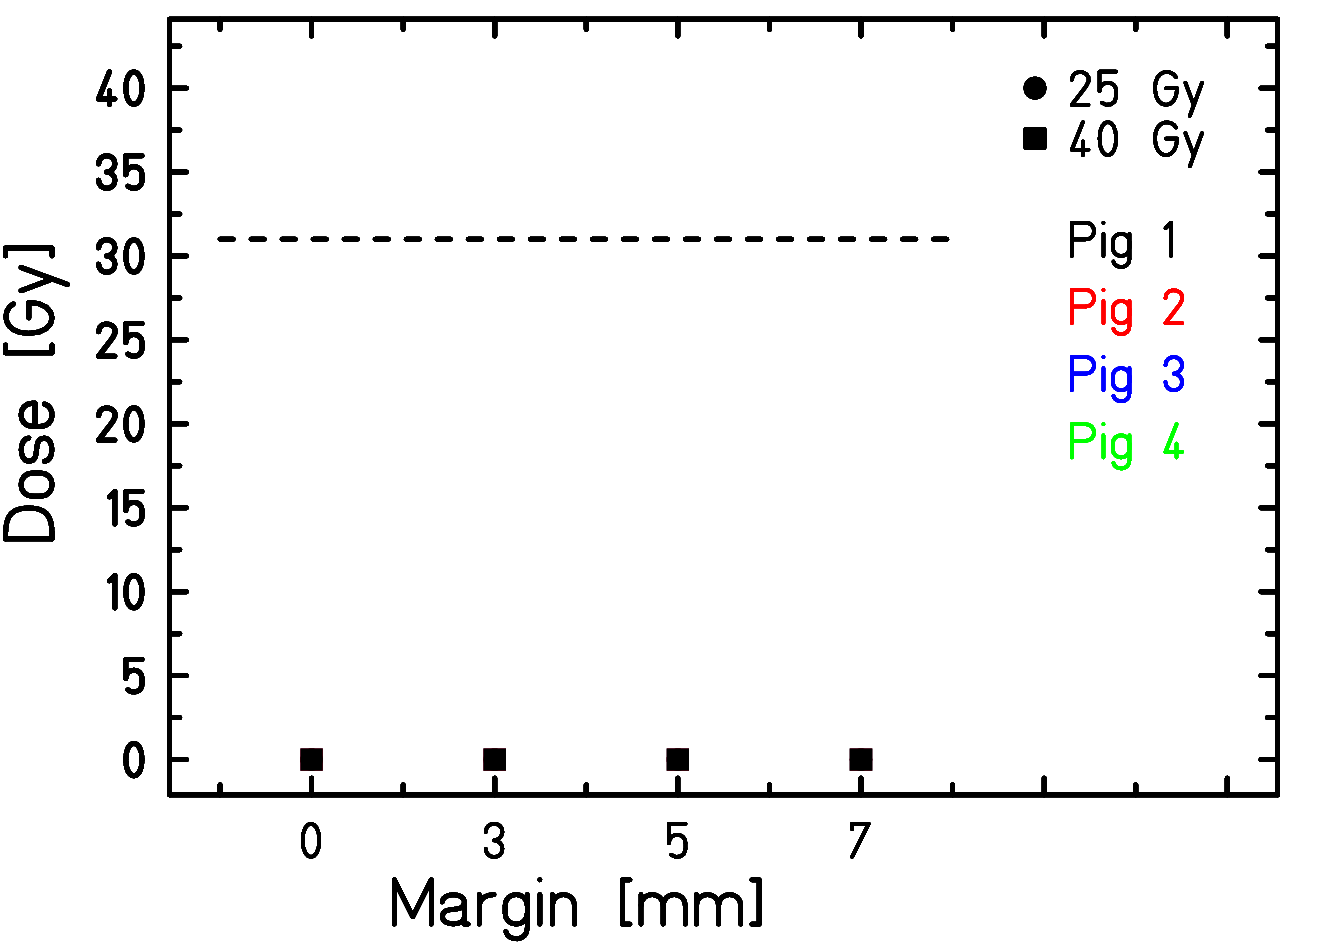
\includegraphics[scale=0.18]{Mayo_Porcine_AORTA_IPV.png}
% %  }
% %  \subfigure[Dose to esophagus]{
% %  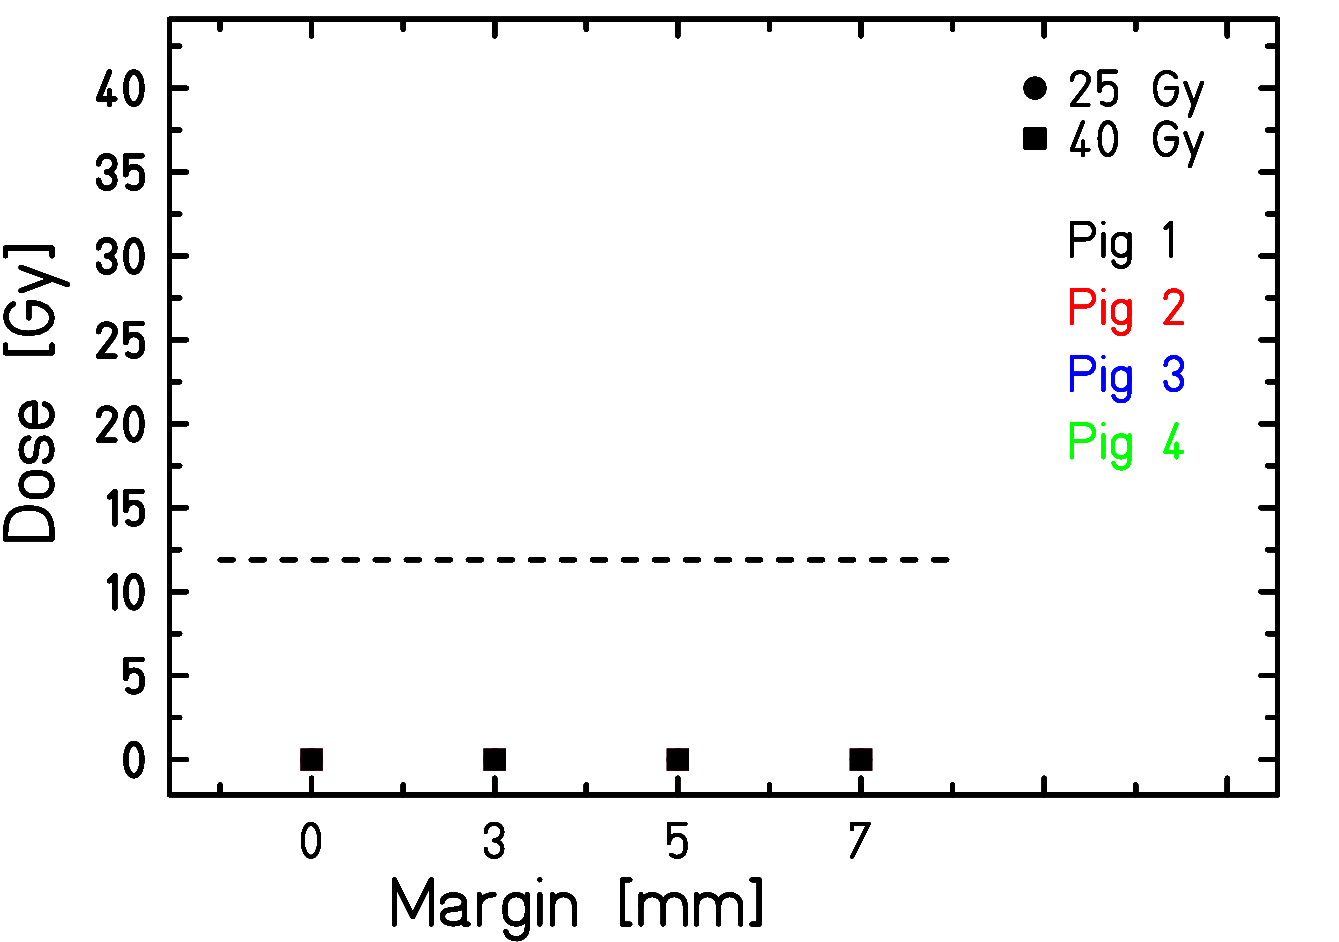
\includegraphics[scale=0.18]{Mayo_Porcine_ESO_IPV_alternativeLimit.png}
% %  }
% %   \subfigure[Dose to trachea]{
% %  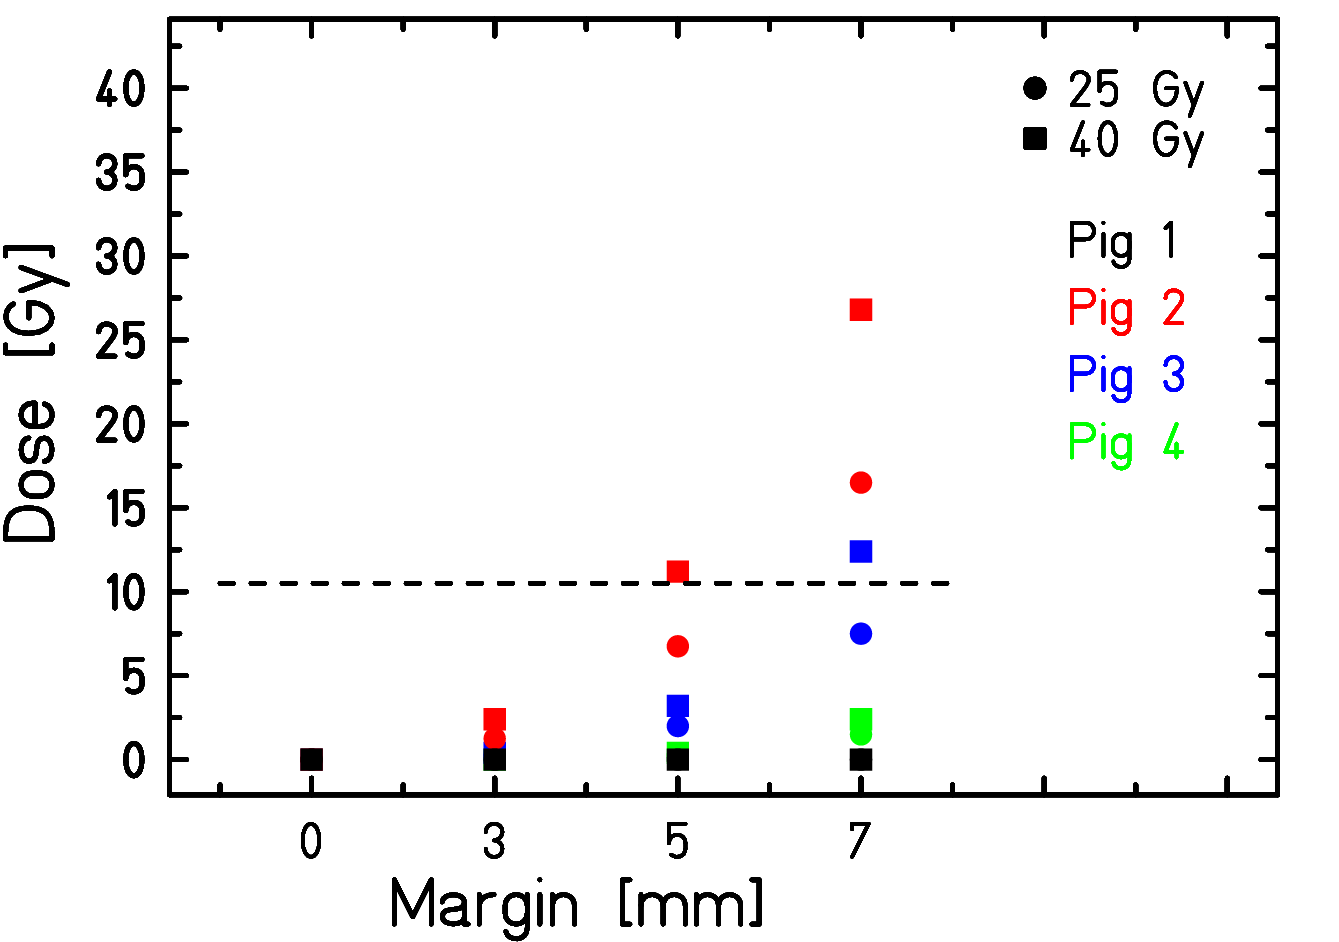
\includegraphics[scale=0.18]{Mayo_Porcine_TRACHEA_IPV.png}
% %  }
% %   \subfigure[Dose to heart]{
% %  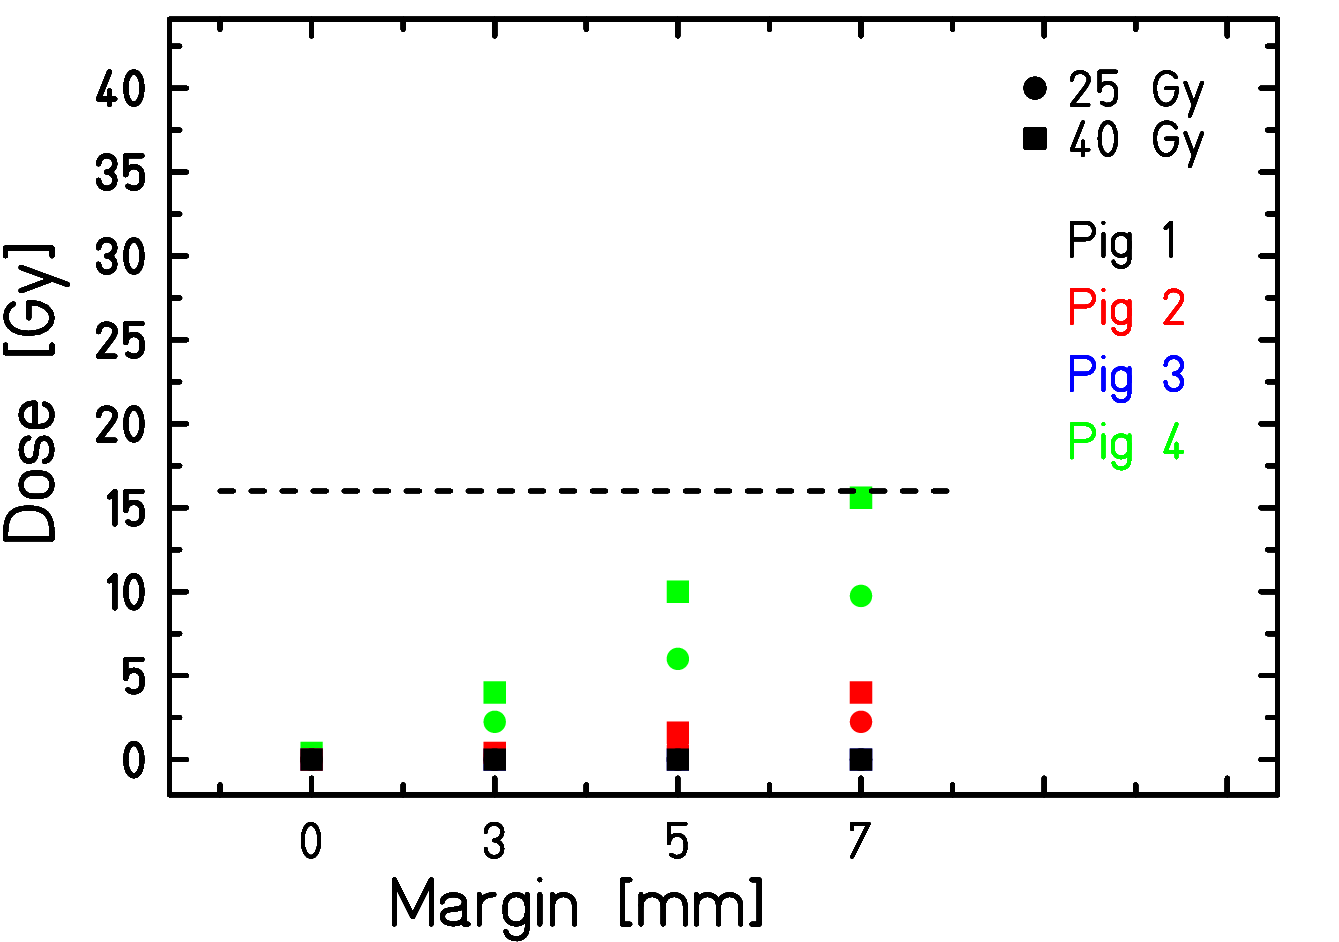
\includegraphics[scale=0.18]{Mayo_Porcine_HEARTwoOverlap_IPV.png}
% %  }
% % \caption{Dose to different OAR when irradiating the IPV in the four porcine data sets (pig 1: black, pig 2: red, pig 3: blue 
% % and pig 4: green) with different margins (0 mm, 3 mm, 5 mm, 7mm) and two different physical doses of 25 Gy and 40 Gy. The dose-volume-limit 
% % for each critical organ is indicated with a dashed line in each plot, respectively.}
% % \label{static_margin_ipv}
% % \end{figure}
% % 
% % \begin{figure}[H]
% % \subfigure[Dose to heart: CTI irradiation]{
% %  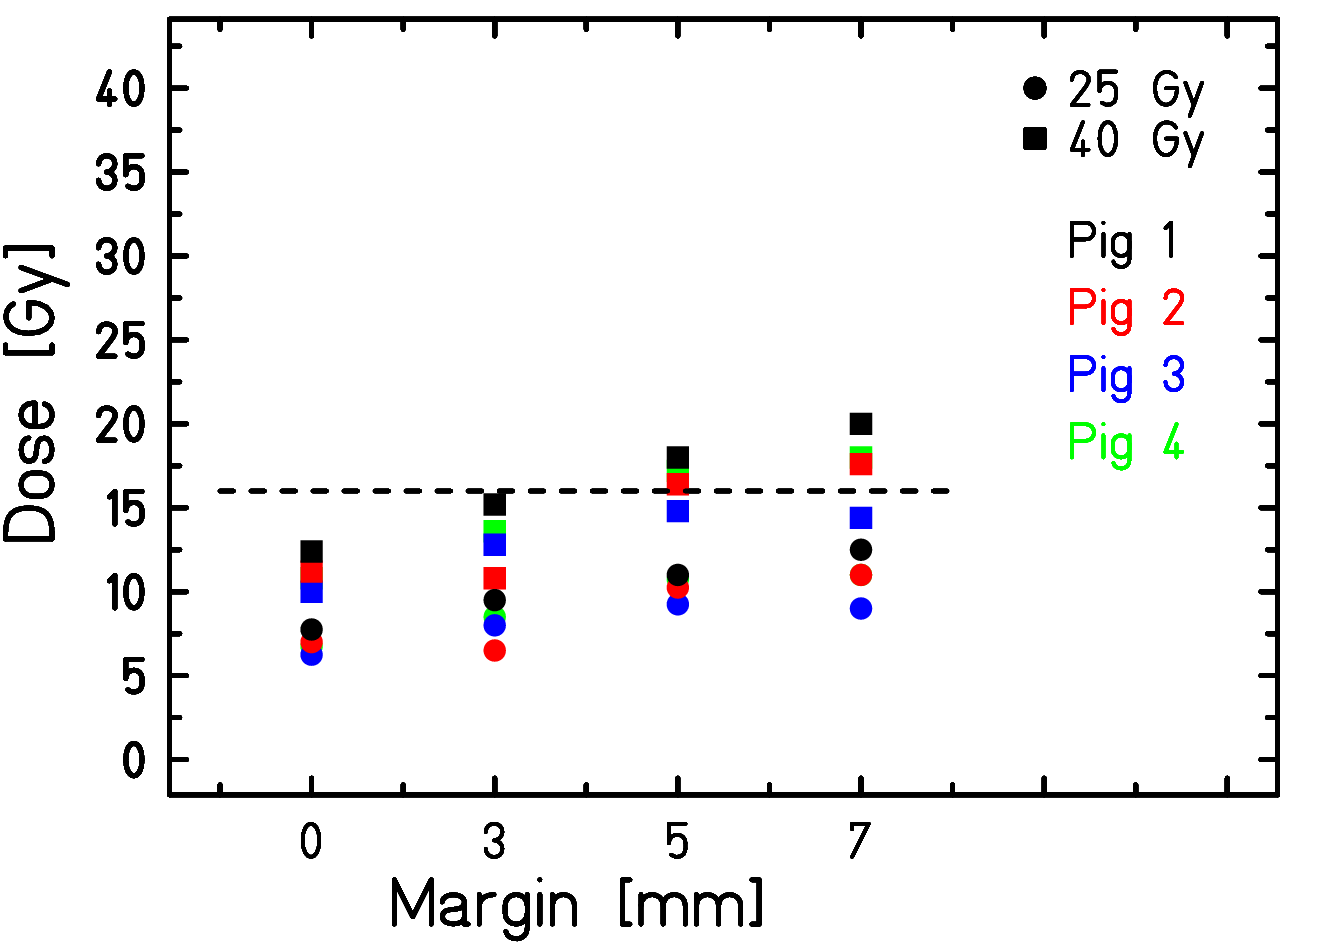
\includegraphics[scale=0.18]{Mayo_Porcine_HEARTwoOverlap_CTI.png}
% %  }
% %   \subfigure[Dose to heart: AV irradiation]{
% %  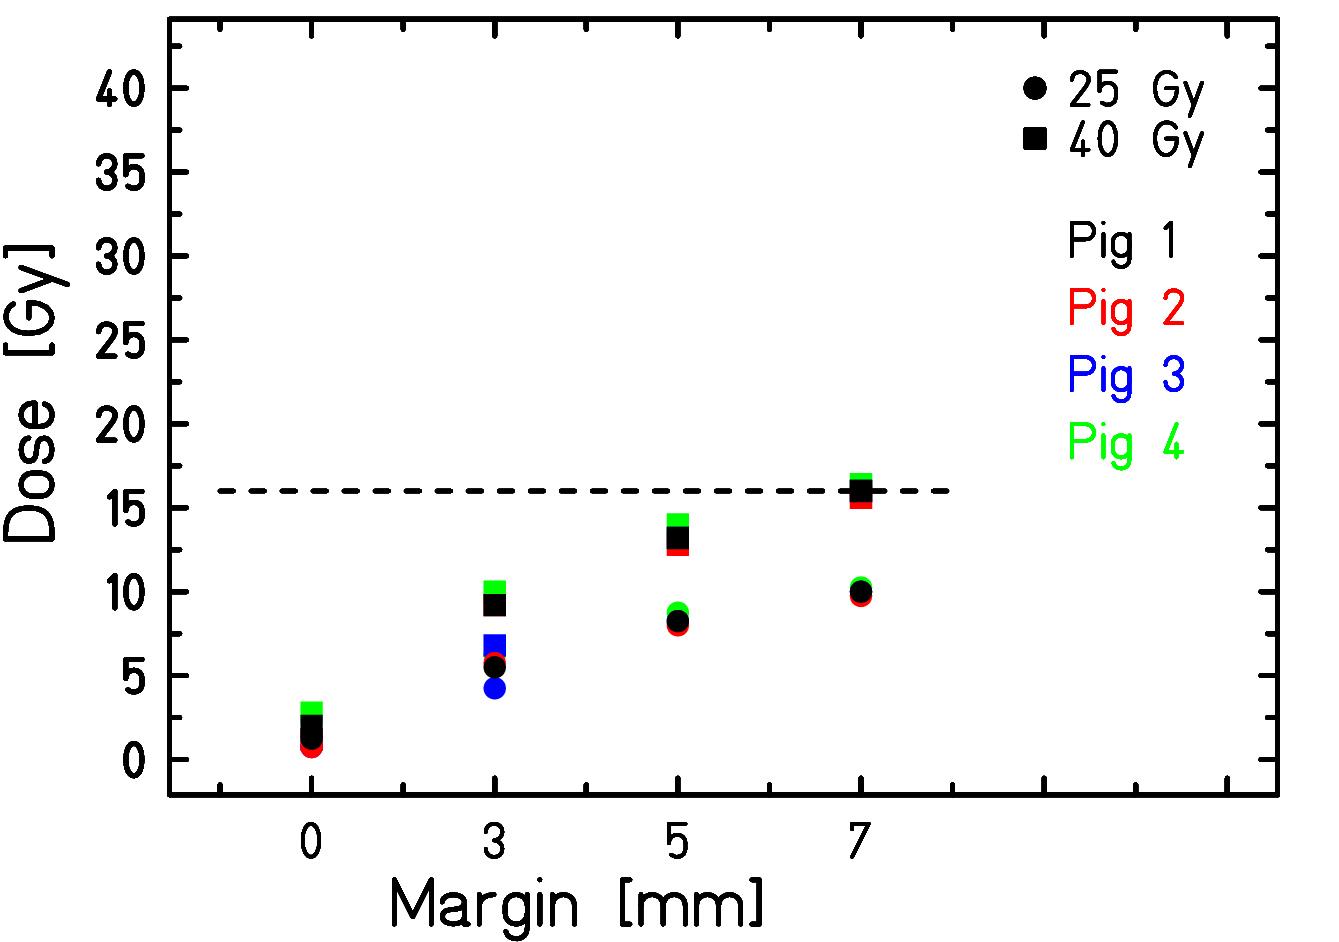
\includegraphics[scale=0.18]{Mayo_Porcine_HEARTwoOverlap_AV.png}
% %  }
% % \caption{Dose to heart when irradiating CTI (left) and AV (right) in the four porcine data sets (pig 1: black, pig 2: red, pig 3: blue 
% % and pig 4: green). Different margins (0 mm, 3 mm, 5 mm, 7mm) for the respective target and two different physical doses of 25 Gy and 40 Gy 
% % were studied. The dose-volume-limit for the heart is indicated with a dashed line.  }
% % \label{static_margin_cti_av}
% % \end{figure}
% % 
% % 
% % For all studied cases, a PTV margin of 3 mm seems to yield robust results which does not exceed dose-volume-limits to close-by organs at risk. 
% % 
% % 
% % % \newpage

\subsection{Motion directions and magnitude}

%%%%%%% HEART BEAT %%%%%%



\begin{figure}[H]
\begin{center}
 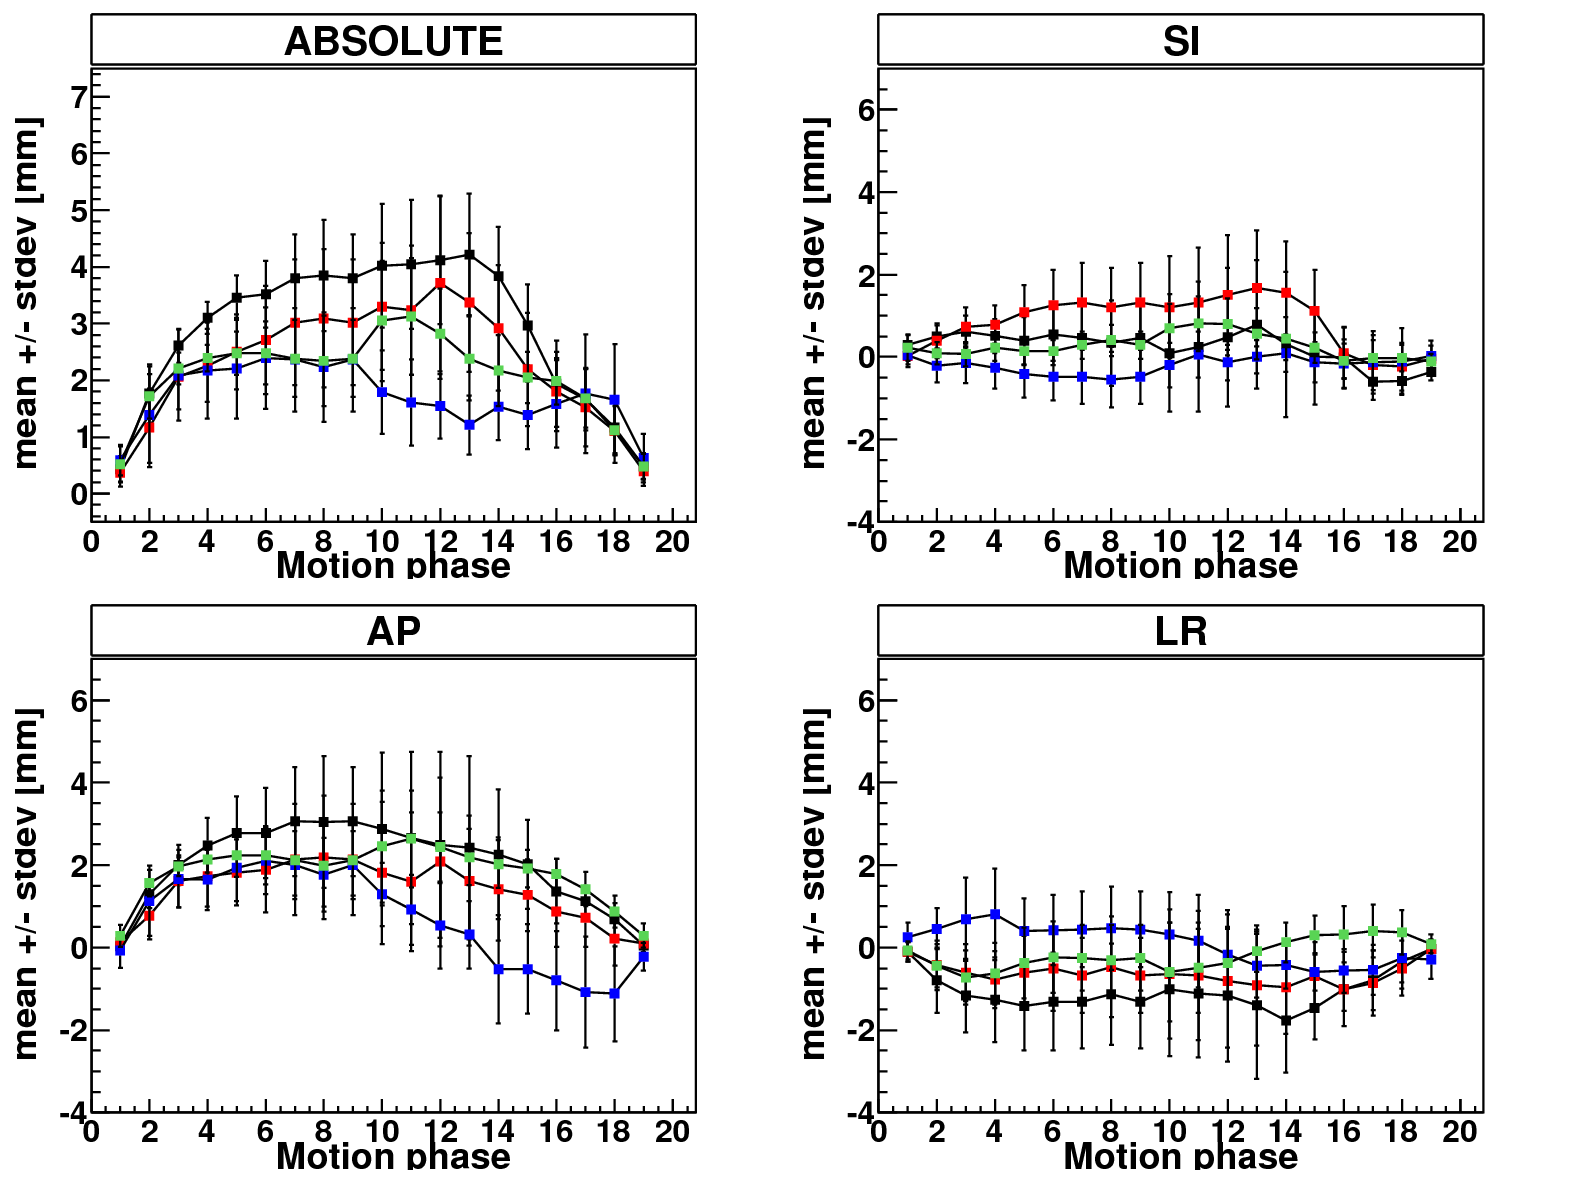
\includegraphics[scale=0.3]{Mayo_PV_HB.png}
\caption{Motion amplitude of PVs under influence of heartbeat for all porcine. (pig 1: black, pig 2: red, pig 3: blue, 
pig 4: green) }
\end{center}
\label{motion_hb_all_pv}
\end{figure}

\begin{figure}[H]
\begin{center}
 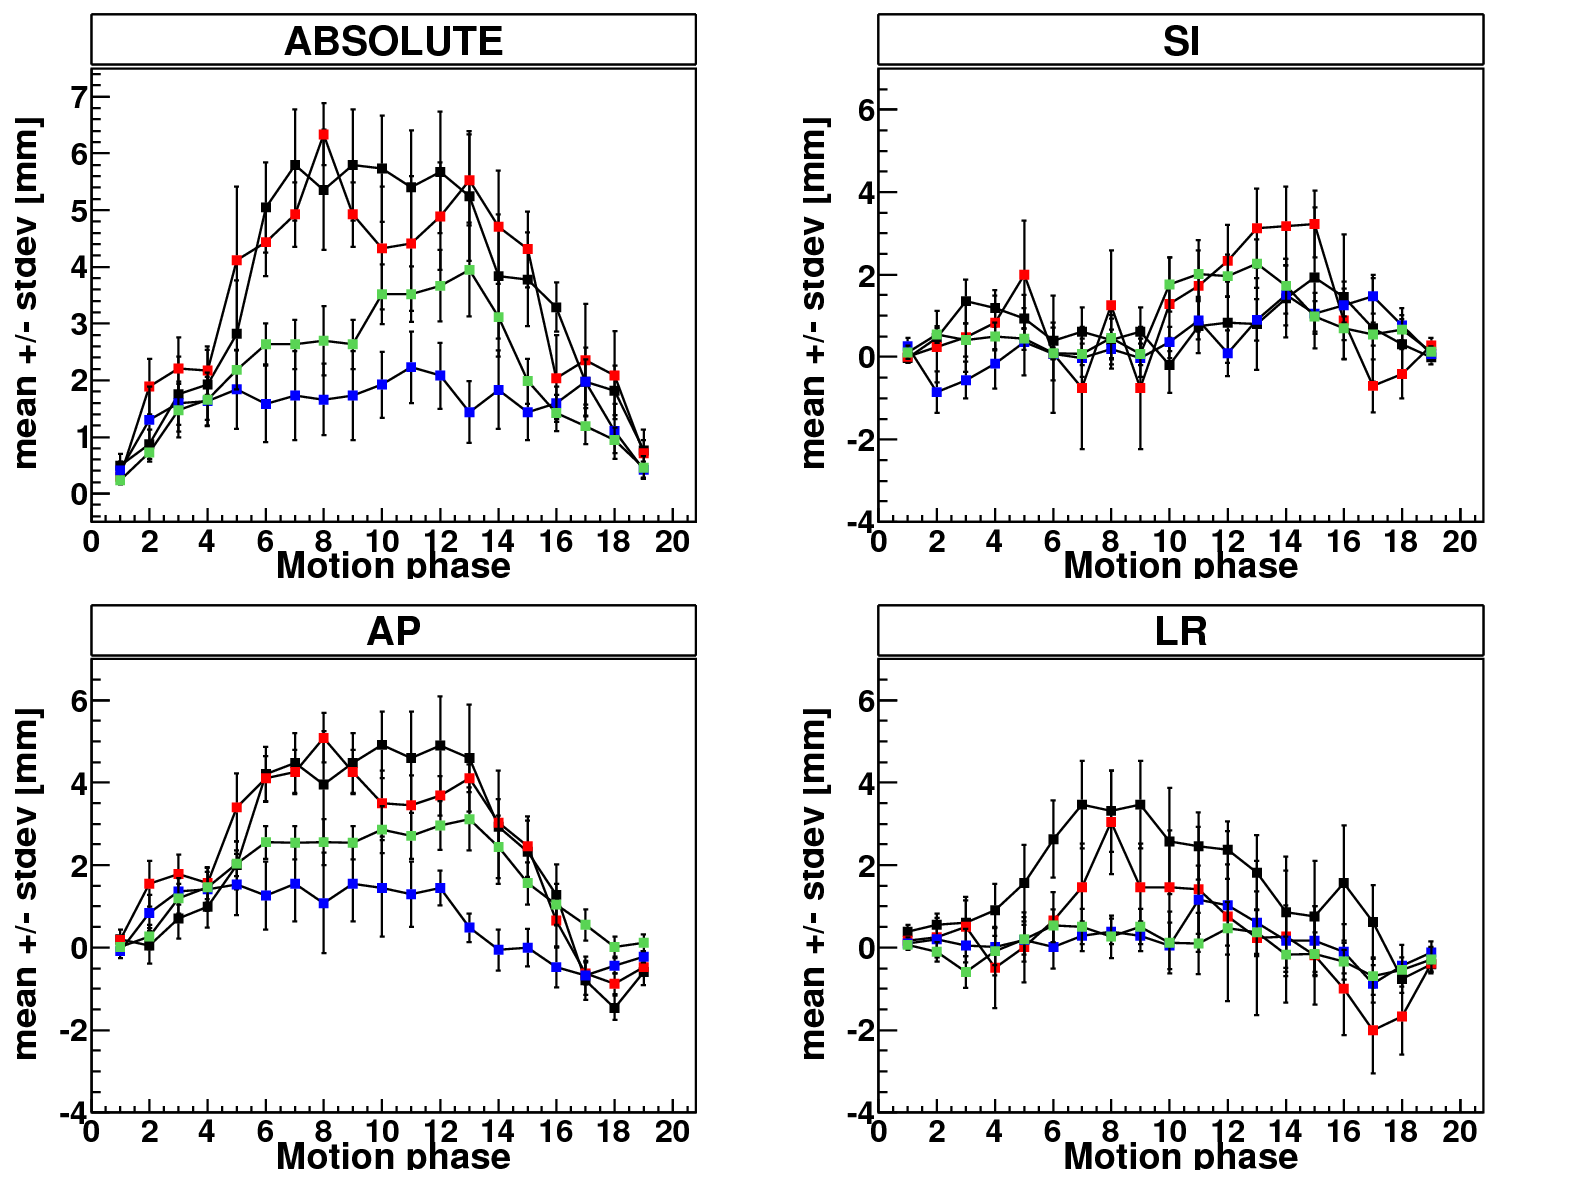
\includegraphics[scale=0.3]{Mayo_CTI_HB.png}
\caption{Motion amplitude of CTI under influence of heartbeat for all porcine. (pig 1: black, pig 2: red, pig 3: blue, 
pig 4: green) }
\end{center}
\label{motion_hb_all_cti}
\end{figure}

\begin{figure}[H]
\begin{center}
 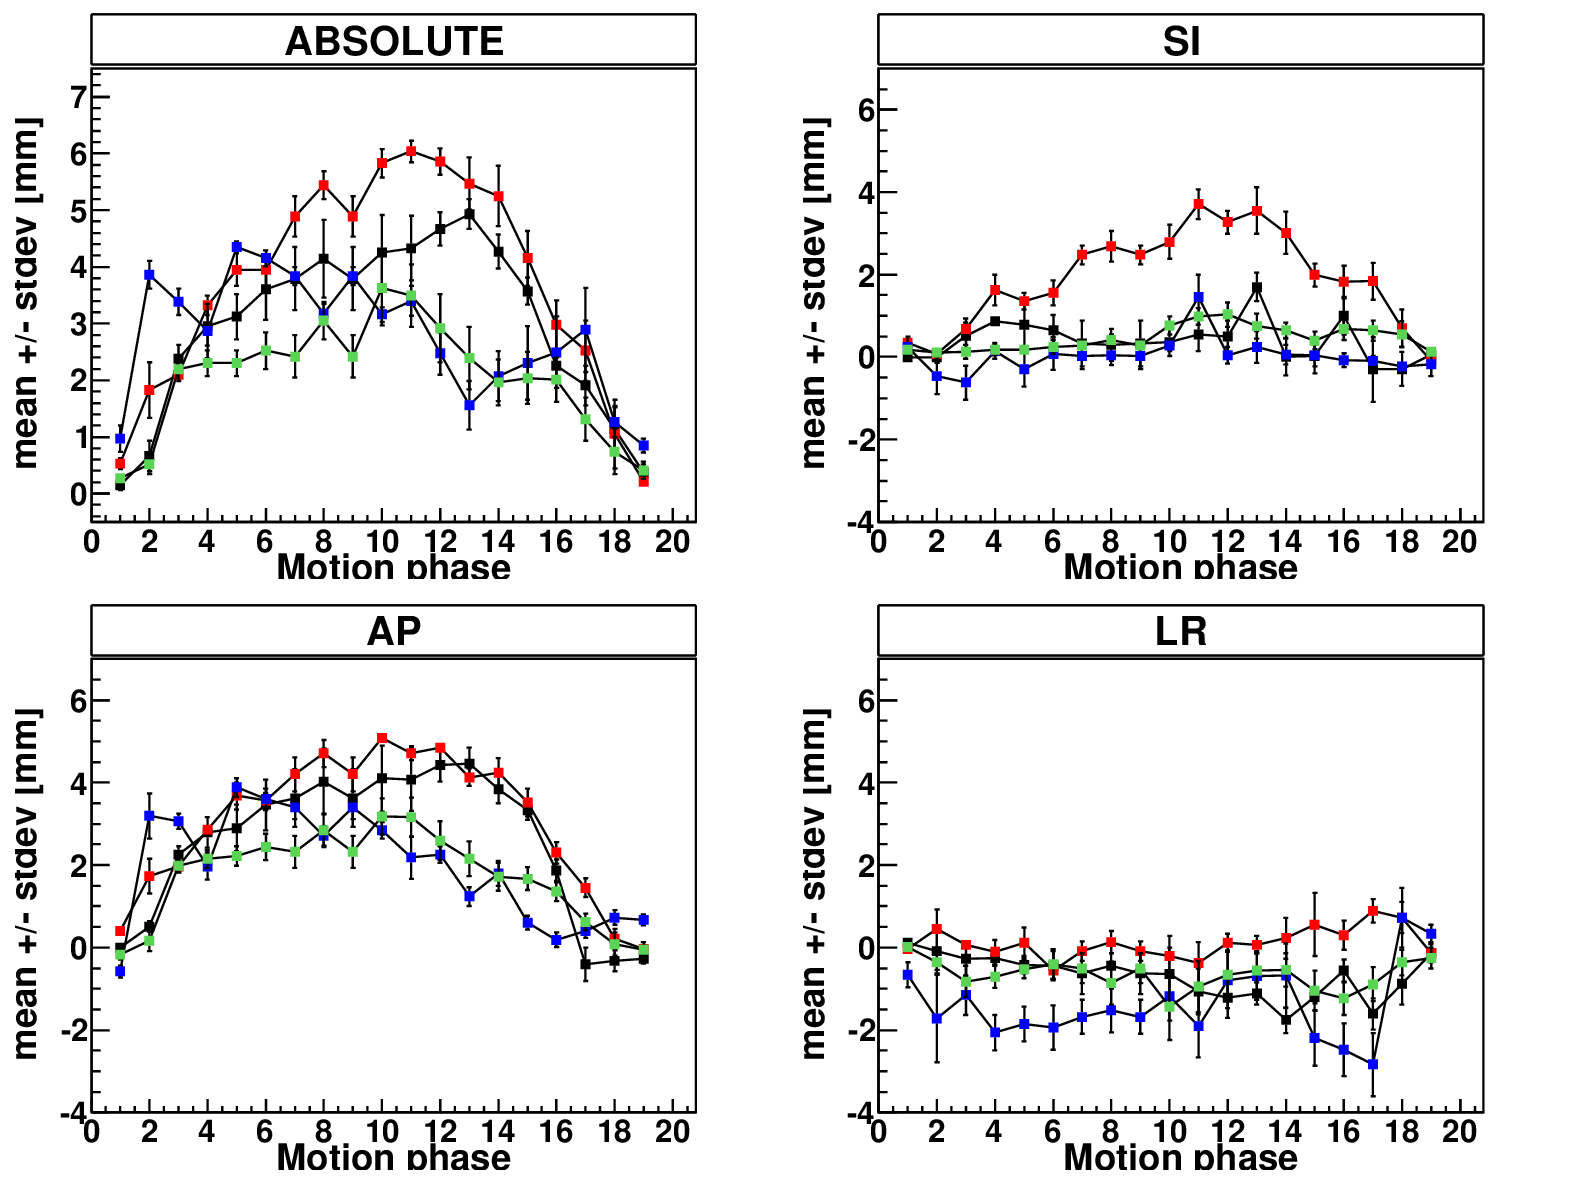
\includegraphics[scale=0.3]{Mayo_AV_HB.png}
\caption{Motion amplitude of AV node under influence of heartbeat for all porcine. (pig 1: black, pig 2: red, pig 3: blue, 
pig 4: green) }
\end{center}
\label{motion_hb_all_av}
\end{figure}

% \subsubsection{Respiration}


%%%%%%%%%%%%%%%%%%%%%%%%%%%%%%%%%%%%%%%%%%%%%%%%%%%%%%%%%%%%%%%%%%%%%%%%%%%%%%%%%%%%%%%%%%%%

% % % \begin{figure}[H]
% % % \subfigure[Respiration: IPV and CTI]{
% % %  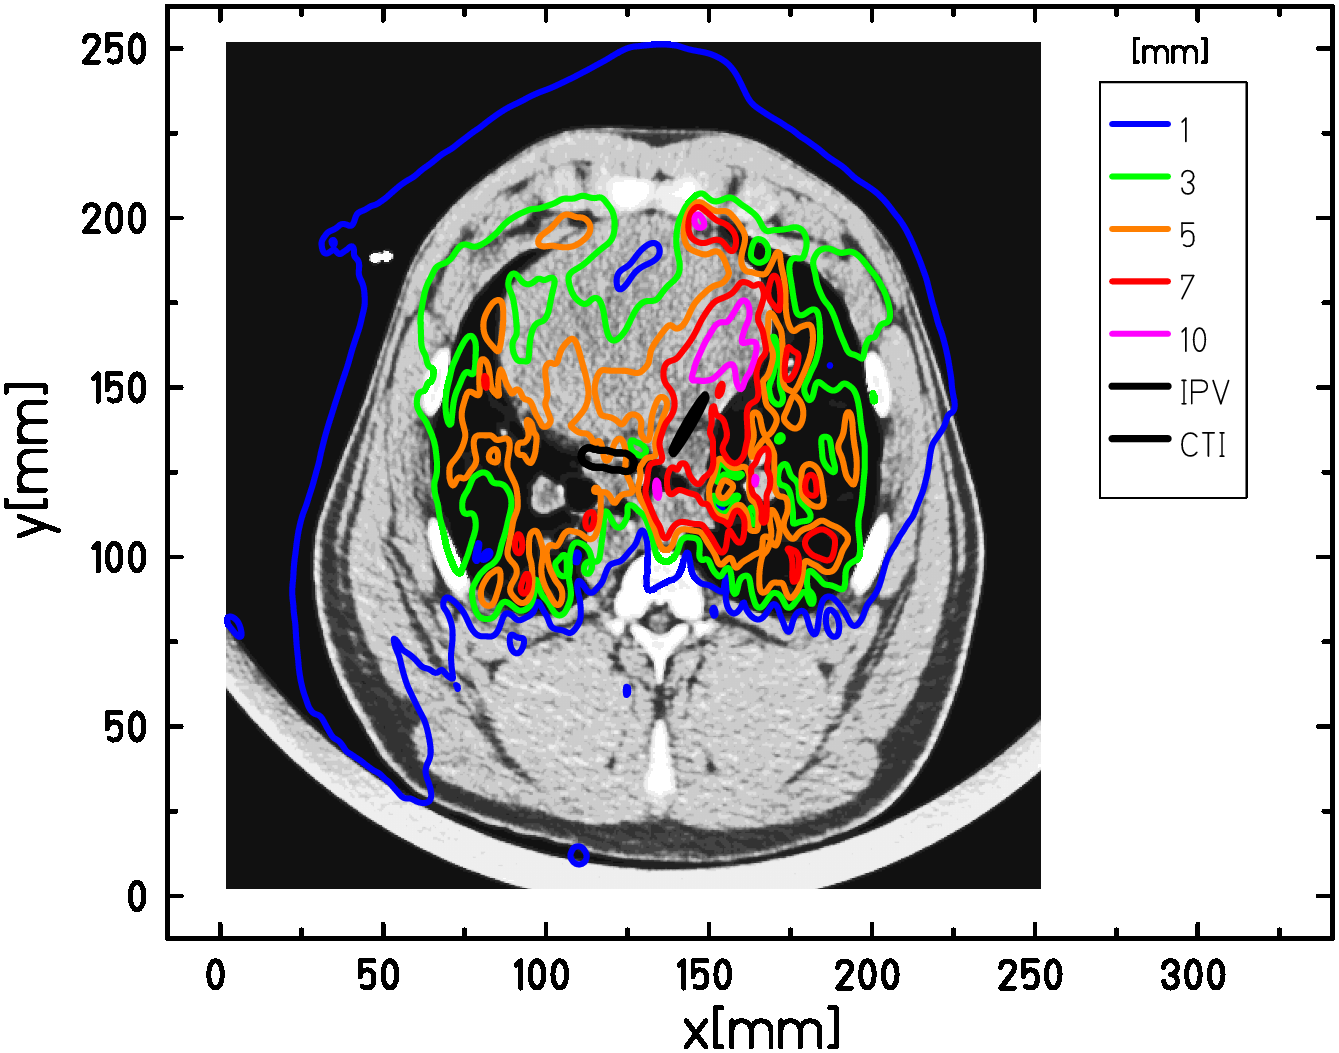
\includegraphics[scale=0.18]{L979_Contour_z_abs_RESP_IPV_CTI_gedreht.png}
% % % }
% % % \subfigure[Respriation: AV]{
% % % 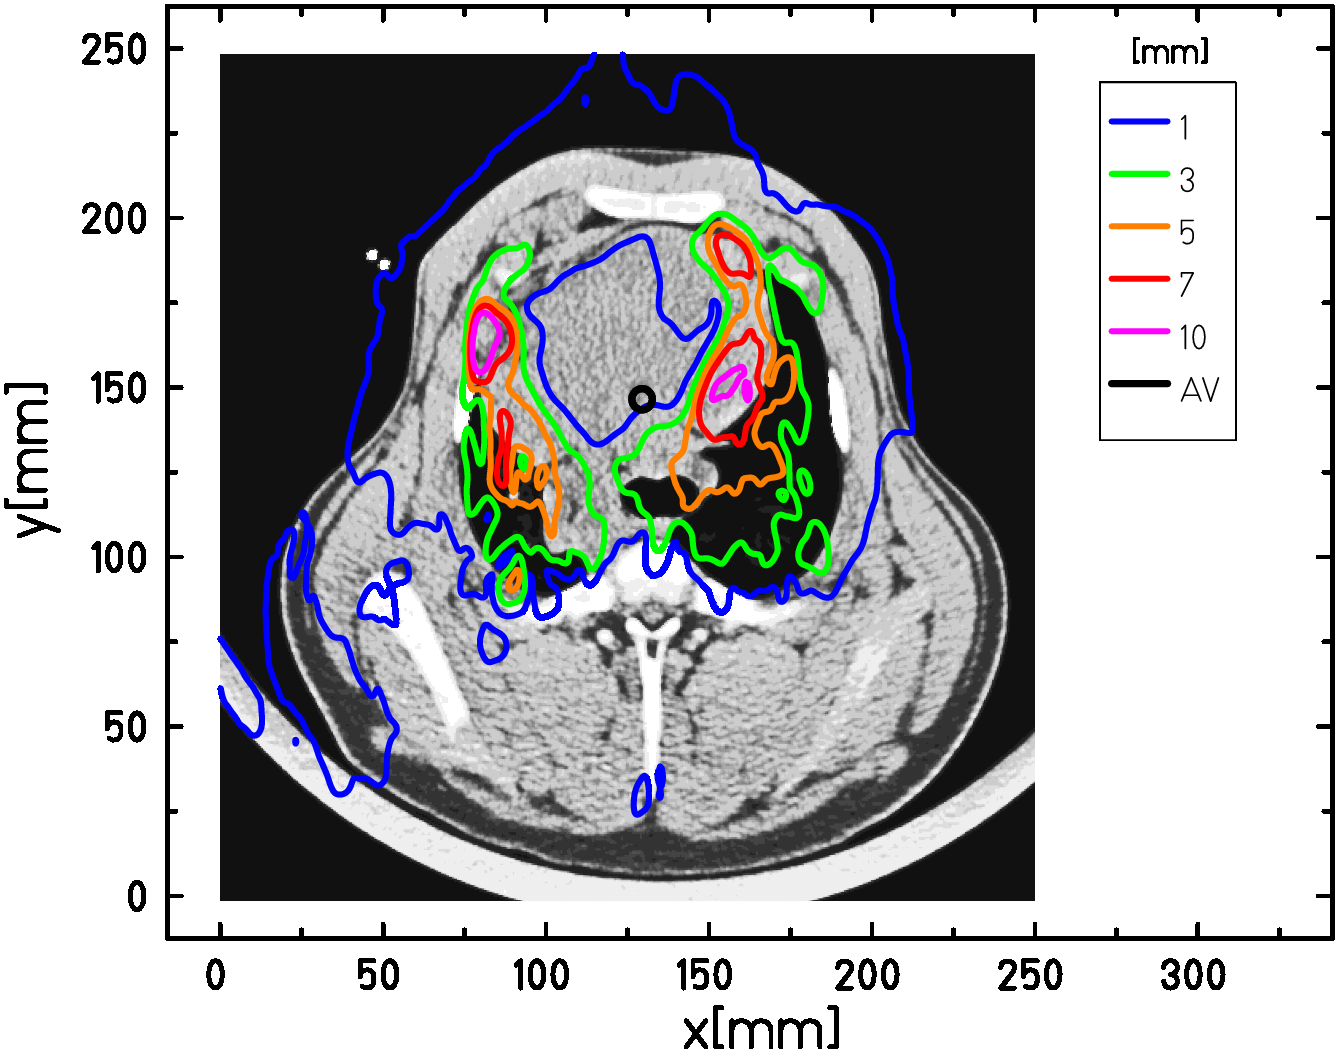
\includegraphics[scale=0.18]{L979_Contour_z_abs_RESP_AV_gedreht.png}
% % % }
% % % \caption{An axial slice of the reference state of the CT overlayed with the absolute values of the displacement vectors (obtained from 
% % % deformable image registration) to the reference phase in the corresponding slice. On the left the displacement influencing IPV and CTI is 
% % % visualised, on the right for AV.}
% % % \label{contour_plot_L979_resp}
% % % \end{figure}
% % % 
% % % 
% % % % % % \begin{figure}[H]
% % % % % % \subfigure[IPV]{
% % % % % %  \includegraphics[scale=0.2]{Mayo_IPV_RESP.png}
% % % % % %  }
% % % % % %   \subfigure[CTI]{
% % % % % %  \includegraphics[scale=0.2]{Mayo_CTI_RESP.png}
% % % % % %  }
% % % % % %    \subfigure[AV]{
% % % % % %  \includegraphics[scale=0.2]{Mayo_AV_RESP.png}
% % % % % %  }
% % % % % % \caption{Motion amplitude in each motion phase of respiration. The results for pig 3 are displayed in blue and for pig 4 in green.}
% % % % % % \label{motion_resp_ipv_cti_av}
% % % % % % \end{figure}
% % % 
% % % 
% % % \begin{figure}[H]
% % % \begin{center}
% % %  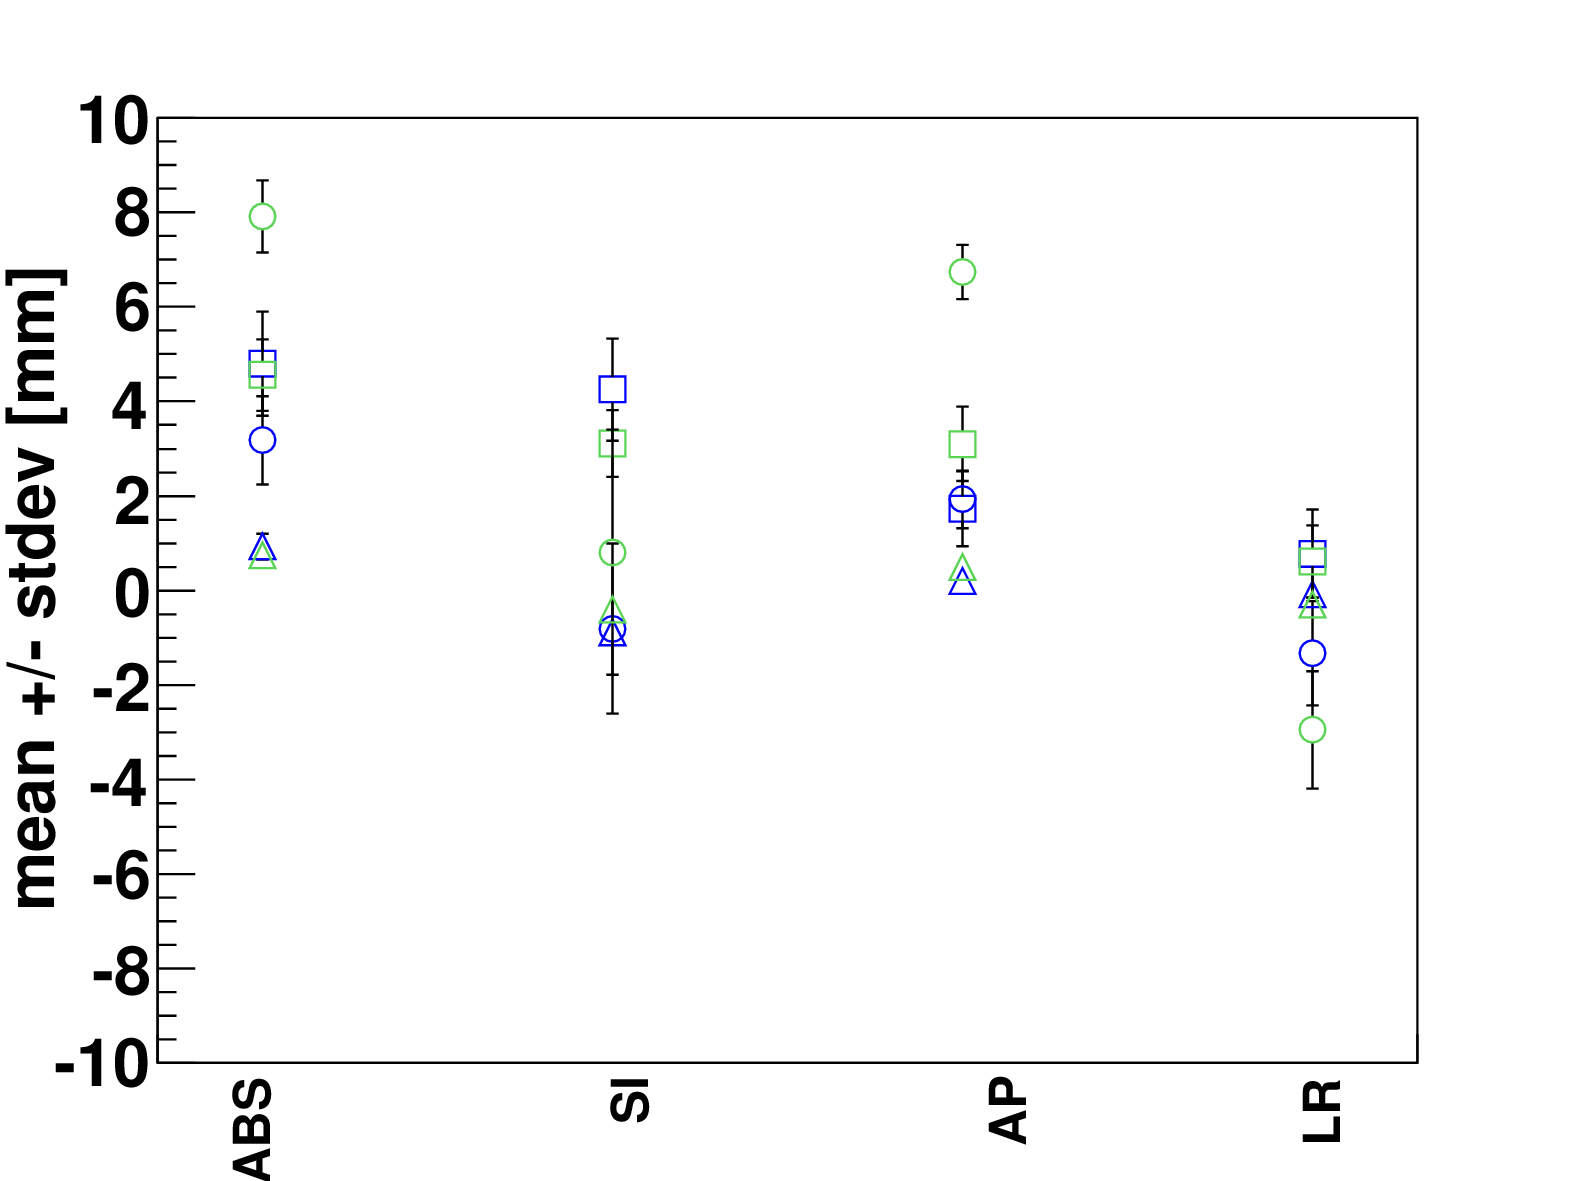
\includegraphics[scale=0.18]{Mayo_ALL_RESP.png}
% % % \caption{Motion amplitude of respiration for all target volumes. IPV motion is symbolised with a square, CTI motion with a circle and AV motion 
% % % with a triangle. (pig 3: blue, pig 4: green) }
% % % \end{center}
% % % \label{motion_resp_ipv_cti_av}
% % % \end{figure}

%%%%%%%%%%%%%%%%%%%%%%%%%%%%%%%%%%%%%%%%%%%%%%%%%%%%%%%%%%%%%%%%%%%%%%%%%%%%%%%%%%%%%%%%%%%%


% \newpage

% \subsubsection{Heart beat}
% 
%%%%%%%%%%%%%%%%%%%%%%%%%%%%%%%%%%%%%%%%%%%%%%%%%%%%%%%%%%%%%%%%%%%%%%%%%%%%%%%%%%%%%%%%%%%%
% % \begin{figure}[H]
% % \subfigure[Heart beat, max motion ventricle: IPV, CTI]{
% %  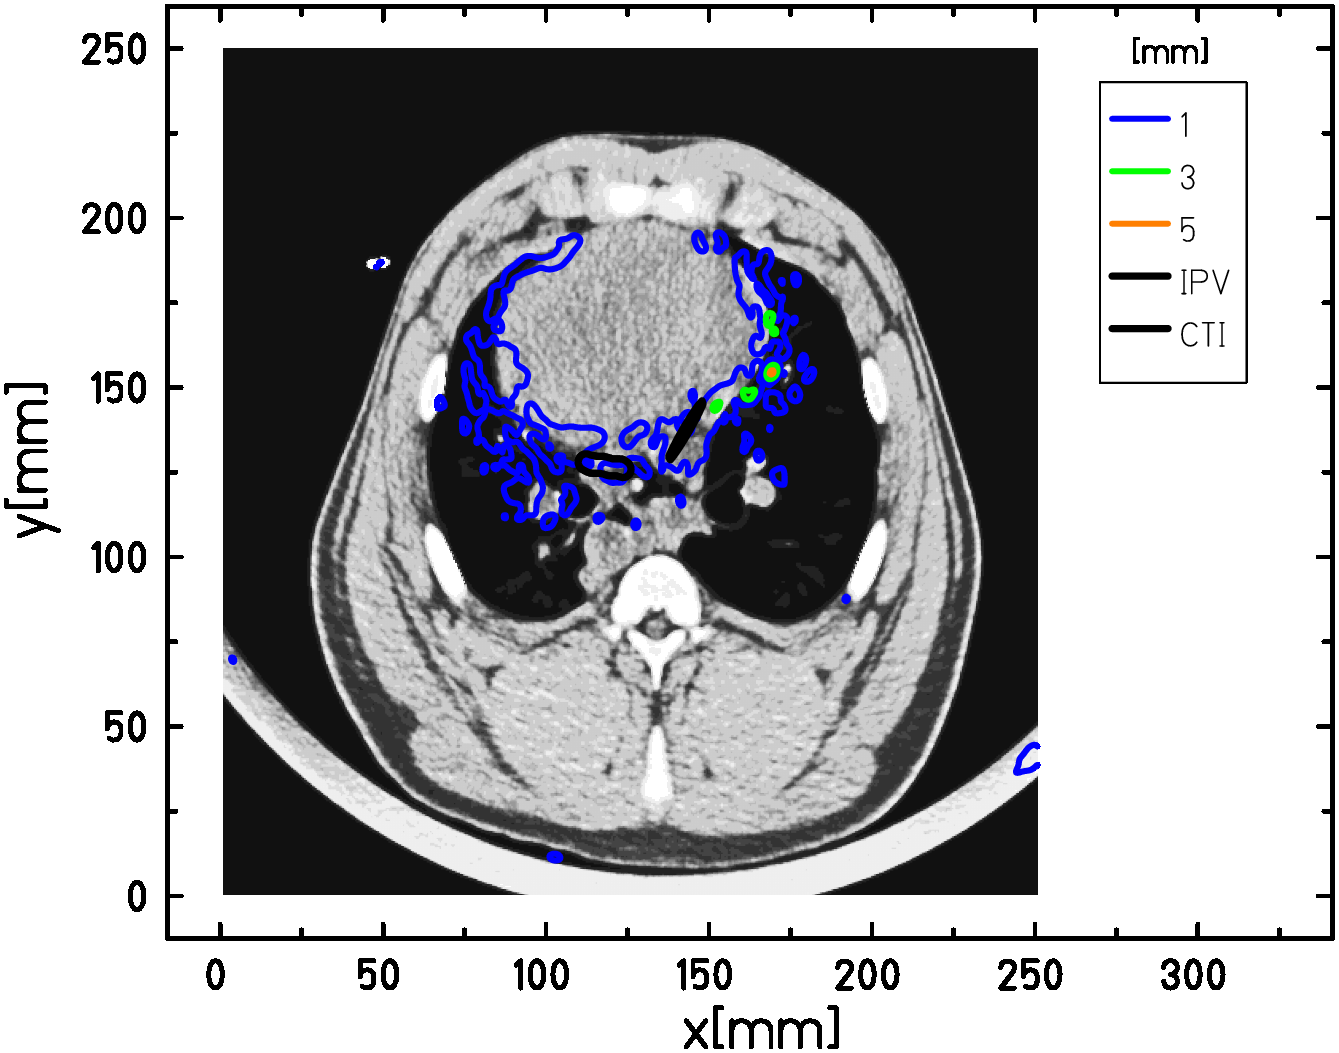
\includegraphics[scale=0.18]{L979_Contour_z_abs_HB_03_IPV_CTI_gedreht.png}
% % }
% % \subfigure[Heart beat, max motion ventricle: AV]{
% % 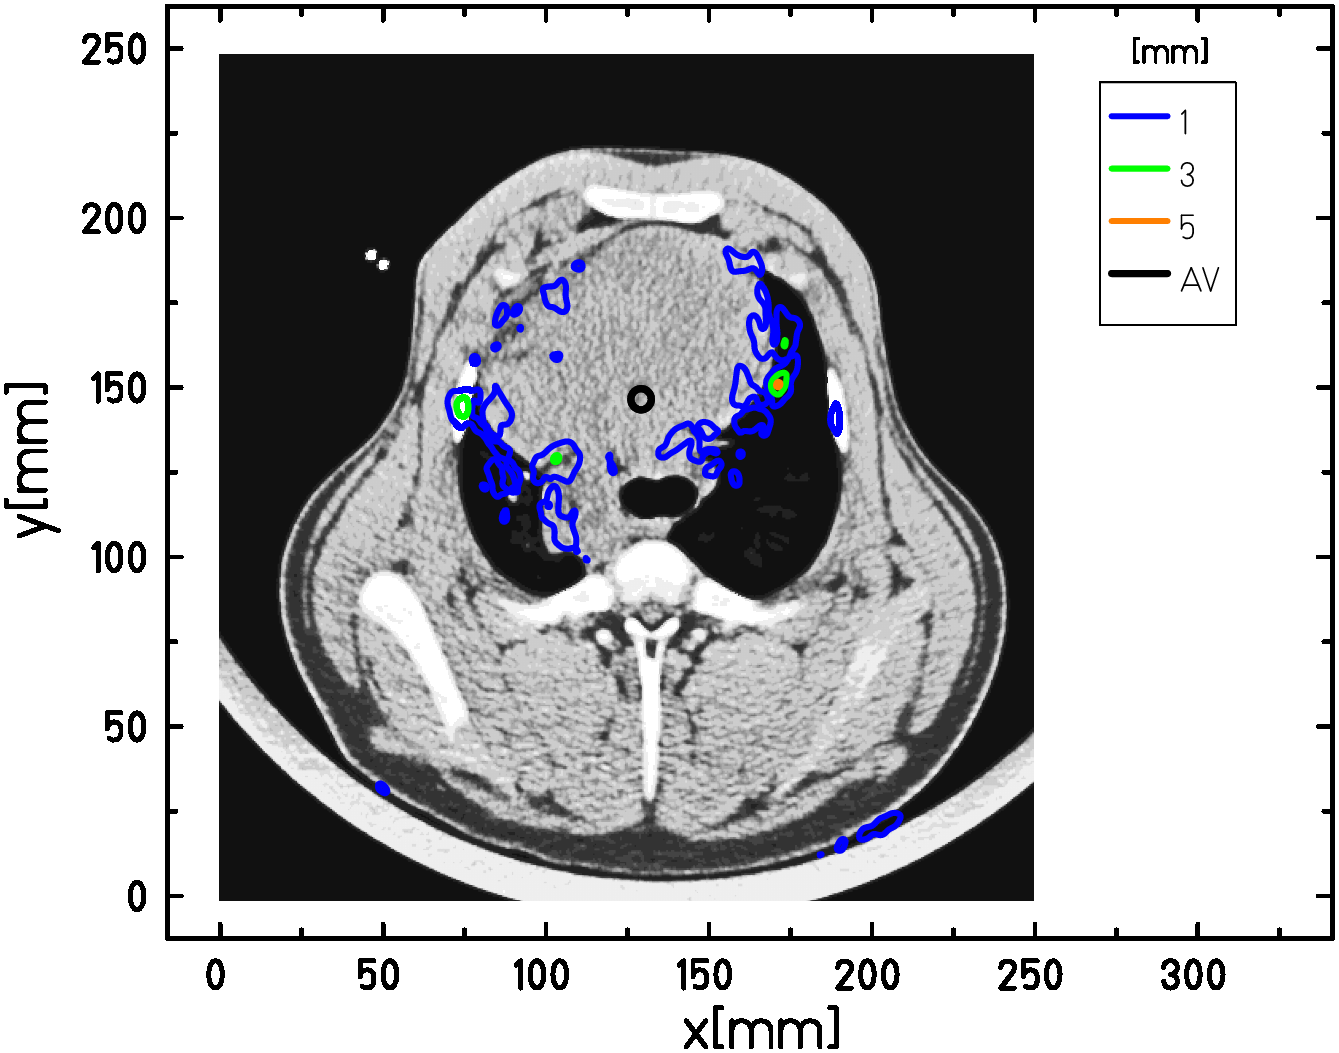
\includegraphics[scale=0.18]{L979_Contour_z_abs_HB_03_AV_gedreht.png}
% % }
% % \subfigure[Heart beat, max motion atria: IPV, CTI]{
% %  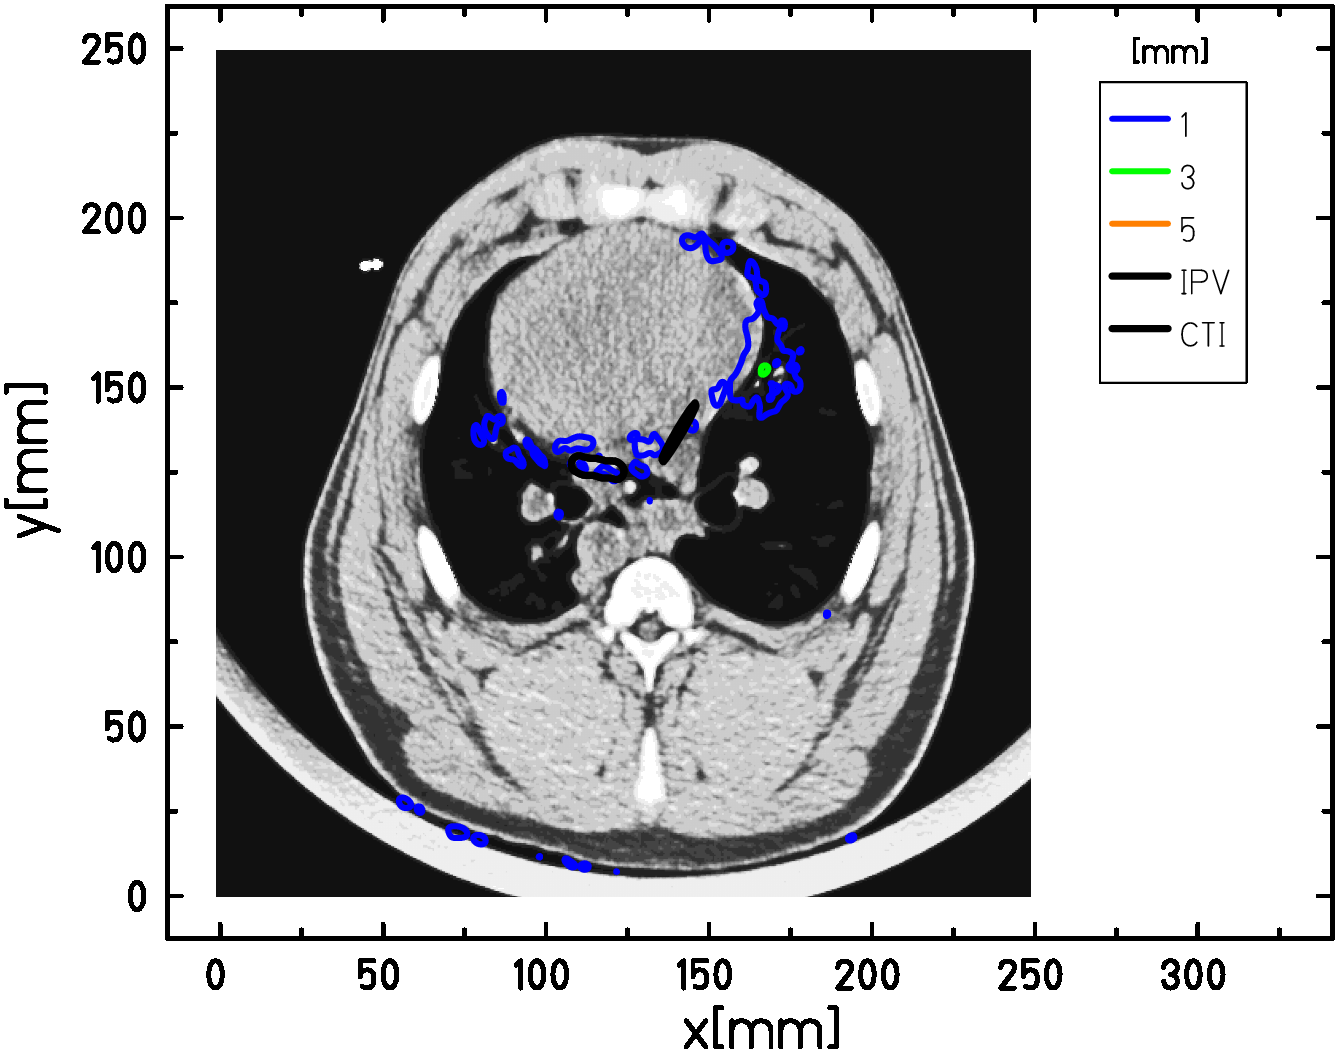
\includegraphics[scale=0.18]{L979_Contour_z_abs_HB_18_IPV_CTI_gedreht.png}
% % }
% % \subfigure[Heart beat, max motion atria: AV]{
% % 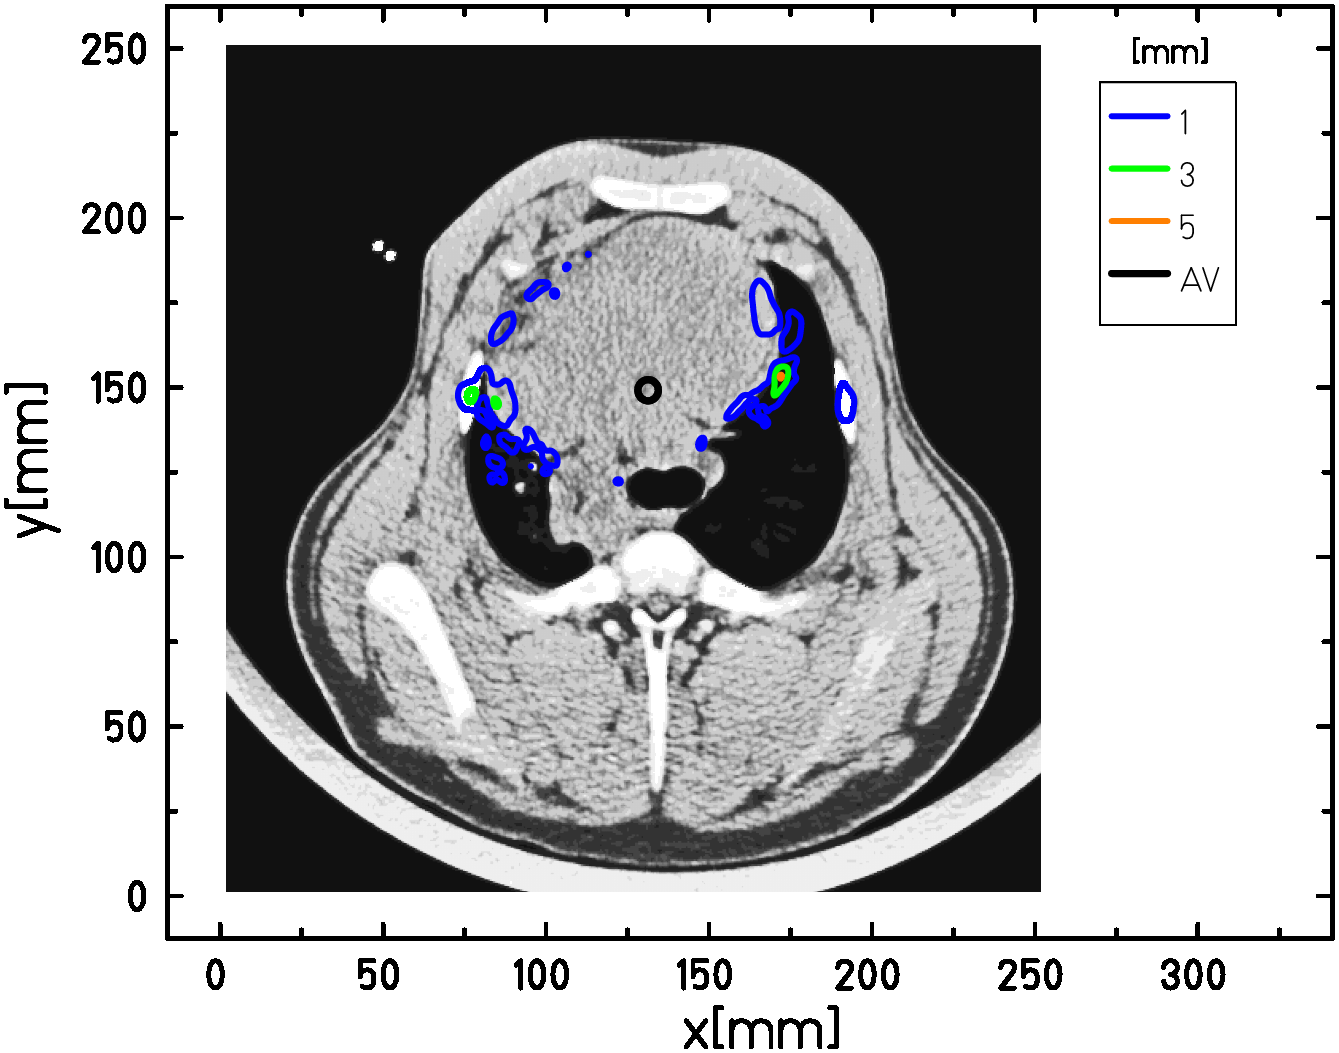
\includegraphics[scale=0.18]{L979_Contour_z_abs_HB_18_AV_gedreht.png}
% % }
% % \caption{Axial slices of the reference state of the CT overlayed with the absolute values of the displacement field (obtained from 
% % deformable image registration) in the corresponding slice for heart beat. In the top row the displacement from the motion phase with the 
% % maximal ventricle motion to the reference phase is shown, in the lower row the displacement from the motion phase with the maximal 
% % atrial motion. On the left the displacement influencing IPV and CTI is visualised, on the right for AV.}
% % \label{contour_plot_L979_hb}
% % \end{figure}
%%%%%%%%%%%%%%%%%%%%%%%%%%%%%%%%%%%%%%%%%%%%%%%%%%%%%%%%%%%%%%%%%%%%%%%%%%%%%%%%%%%%%%%%%%%%

\newpage

% % % \begin{figure}[H]
% % % \begin{center}
% % %  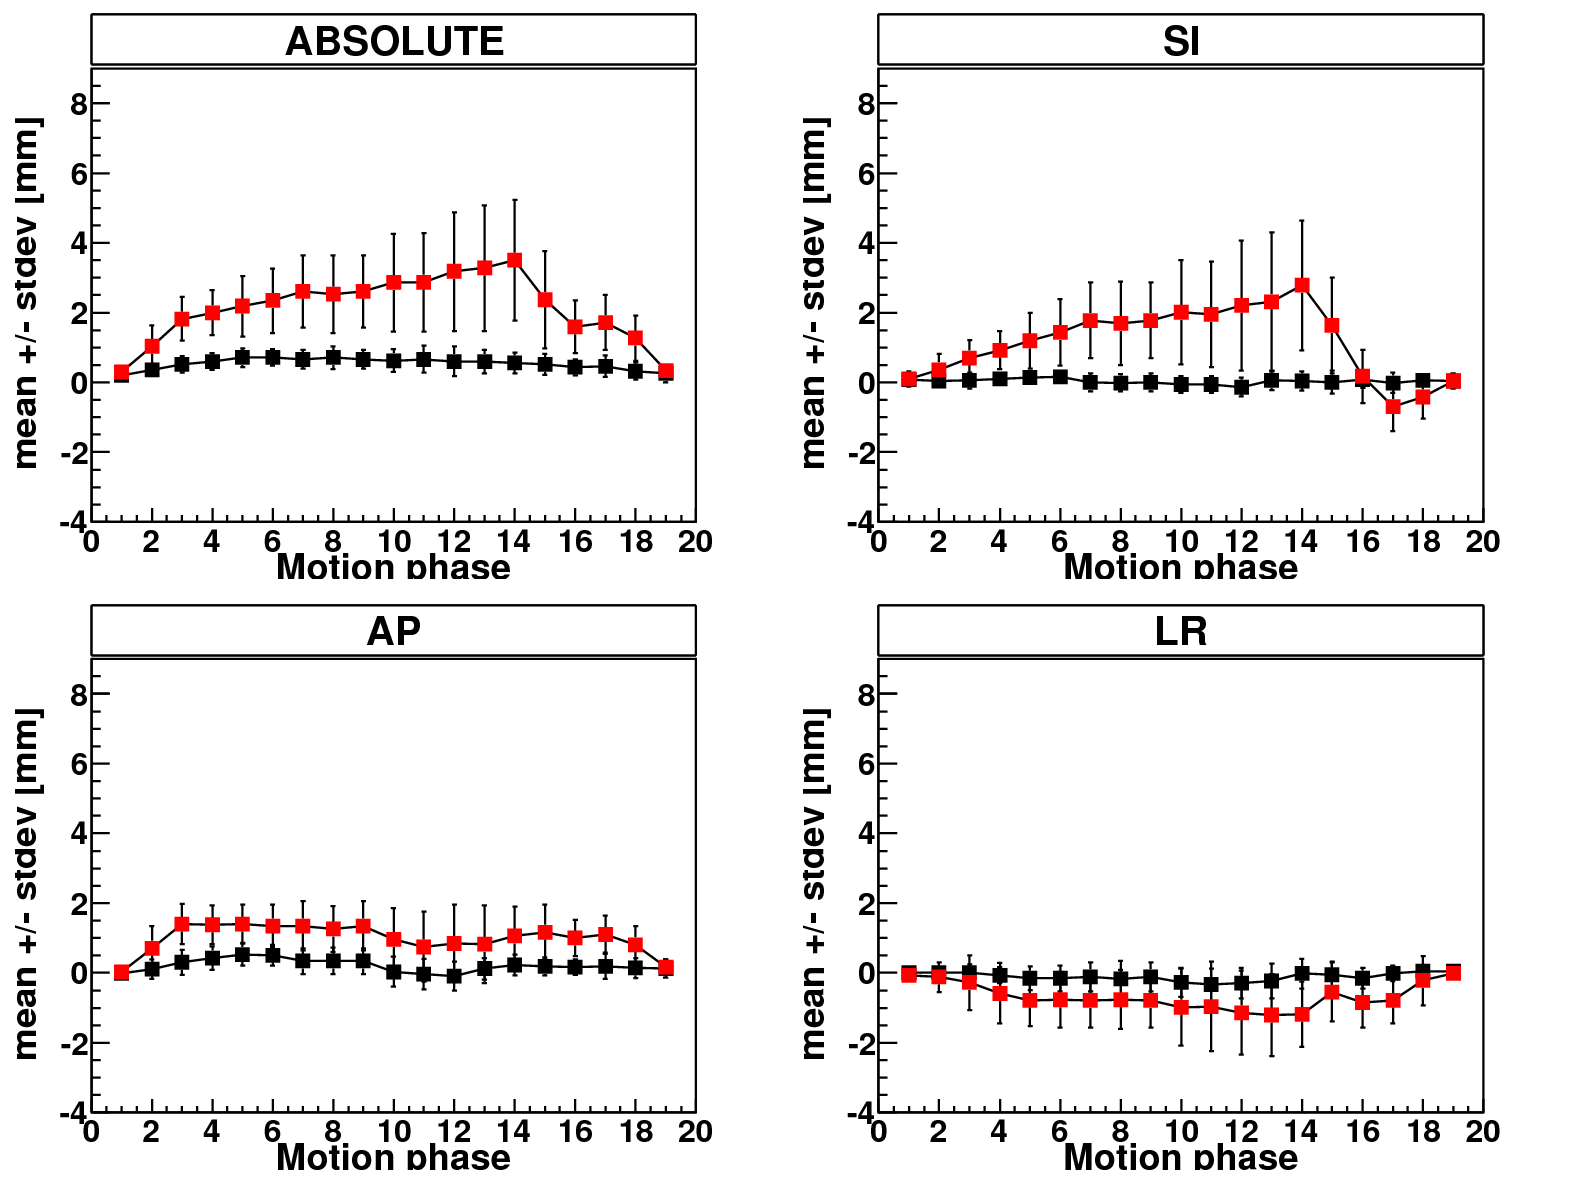
\includegraphics[scale=0.22]{L833_HB_CONTRAST_VS_NATIV_IPV.png}
% % % \caption{IPV: motion amplitude in each motion phase of the heart beat relative to the reference phase. Comparison between native CT data 
% % % (black) and contrast CT (red) for Pig 2.}
% % % \end{center}
% % % \label{motion_hb_ipv}
% % % \end{figure}
% % % 
% % % \begin{figure}[H]
% % % \begin{center}
% % %  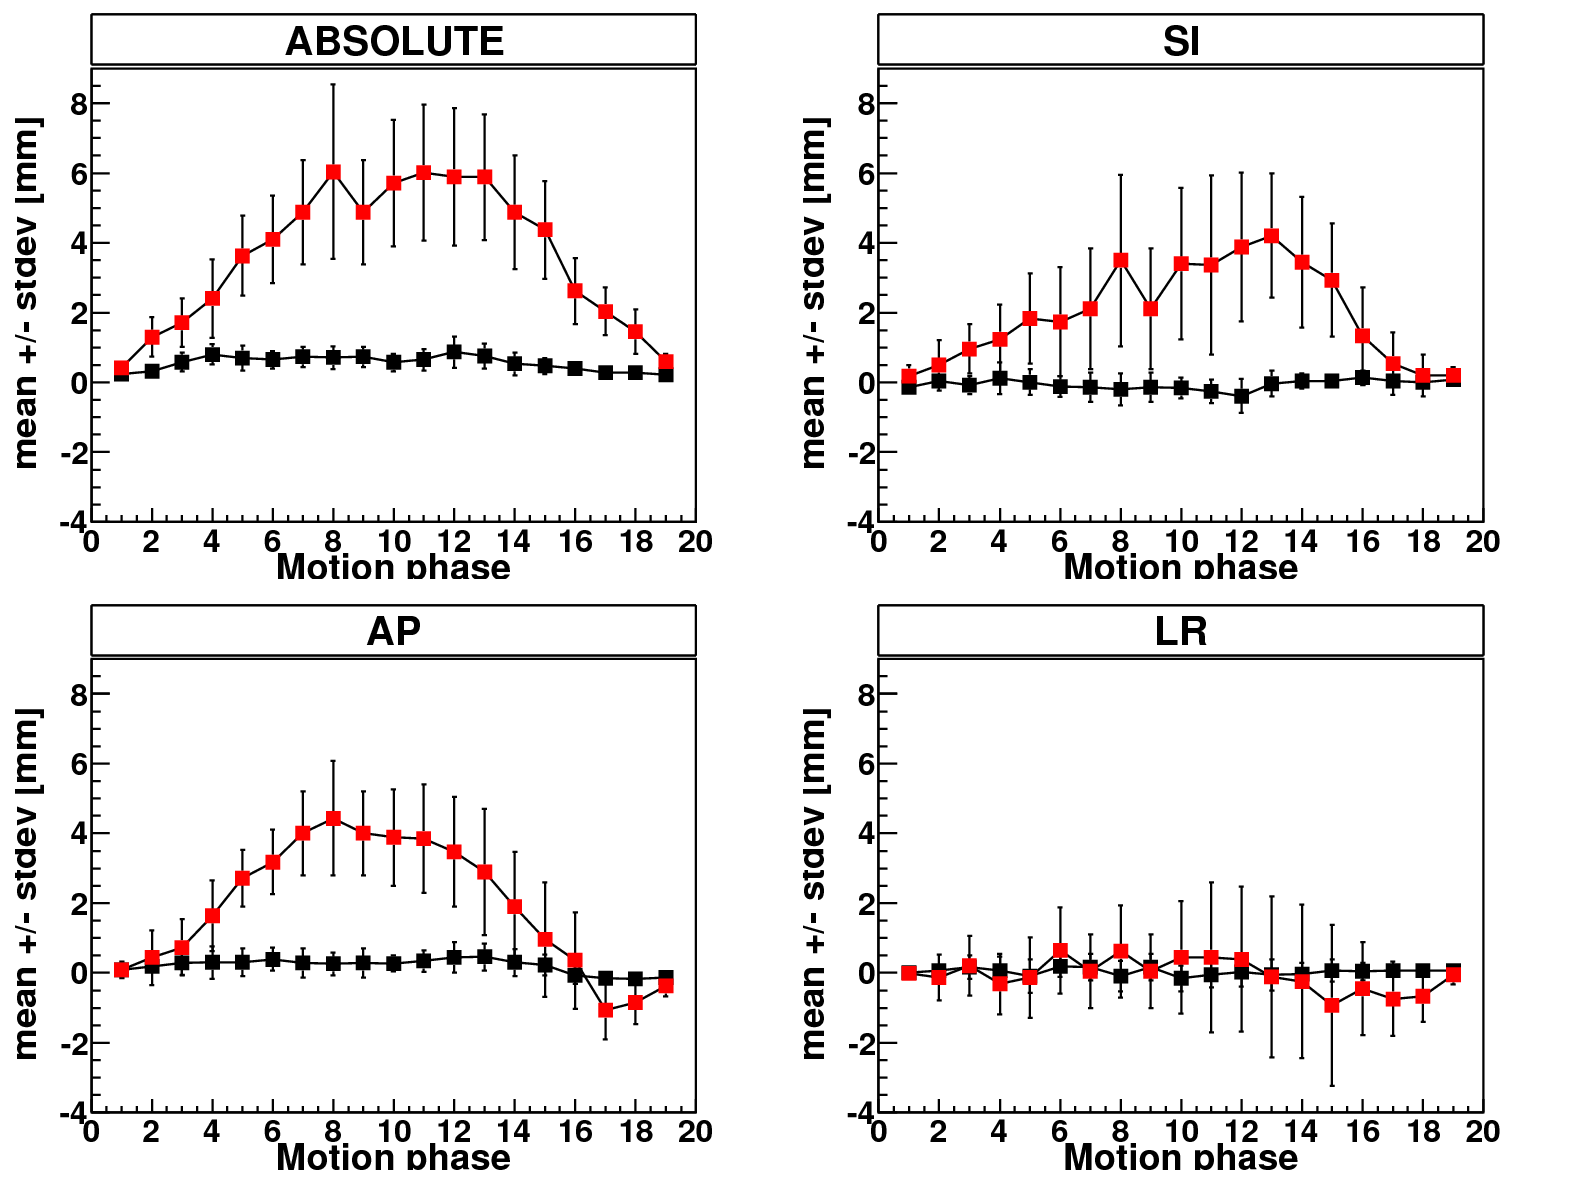
\includegraphics[scale=0.22]{L833_HB_CONTRAST_VS_NATIV_CTI.png}
% % % \caption{CTI: motion amplitude in each motion phase of the heart beat relative to the reference phase. Comparison between native CT data 
% % % (black) and contrast CT (red) for Pig 2.}
% % % \end{center}
% % % \label{motion_hb_cti}
% % % \end{figure}
% % % 
% % % \newpage

% % % \begin{figure}[H]
% % % \begin{center}
% % %  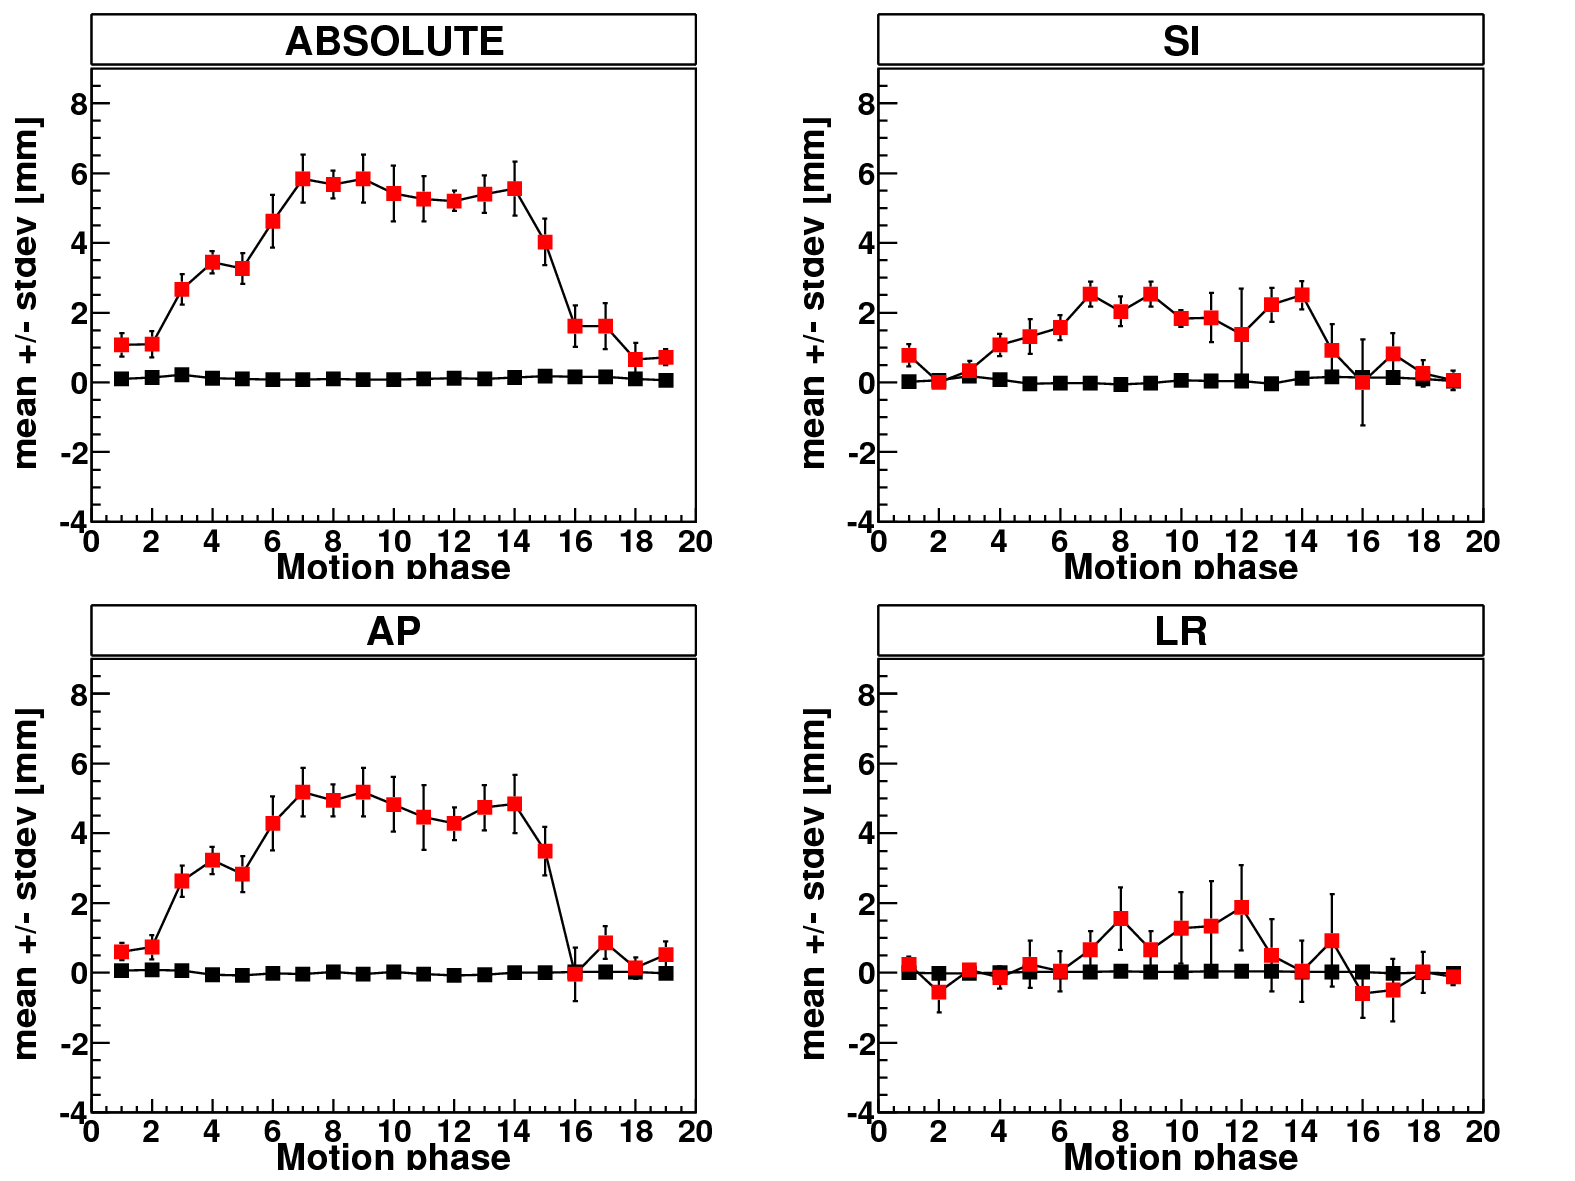
\includegraphics[scale=0.22]{L833_HB_CONTRAST_VS_NATIV_AV.png}
% % % \caption{AV: motion amplitude in each motion phase of the heart beat relative to the reference phase. Comparison between native CT data 
% % % (black) and contrast CT (red) for Pig 2.}
% % % \end{center}
% % % \label{motion_hb_av}
% % % \end{figure}

\begin{figure}[H]
\begin{center}
 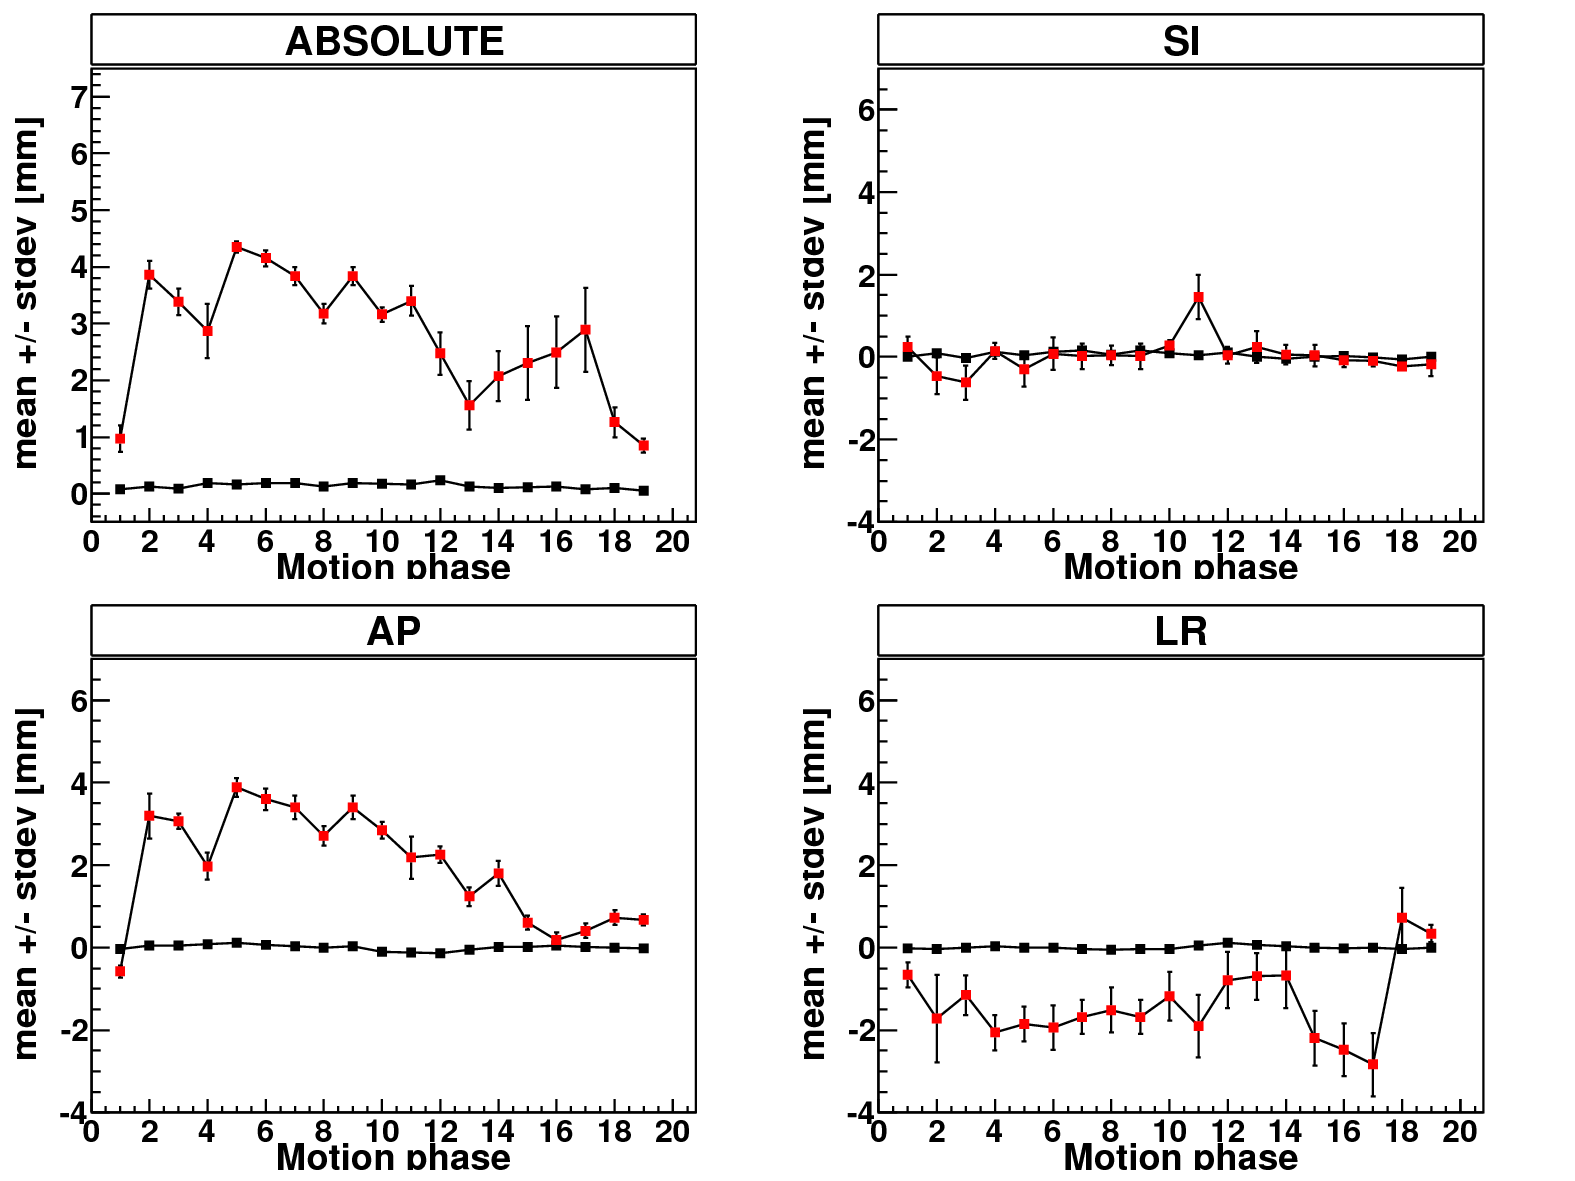
\includegraphics[scale=0.22]{Mayo_AV_NATIV_VS_HB_CONTRAST.png}
\caption{AV: motion amplitude in each motion phase of the heart beat relative to the reference phase. Comparison between native CT data 
(black) and contrast CT (red) for Pig 3.}
\end{center}
\label{motion_hb_av_contrast_nativ}
\end{figure}

- BILD dy von L833: sagittal view -> man sieht das konturen am herzem zwischen nativ und contrast ok!
- large difference between nativ and contrast! naturally ecsp. for targets inside of heart (AV and CTI) \newline 
- IPV: SI largest motion direction \newline
- AV and CTI: AP largest motion direction \newline
- for this pig MP 14 largest motion in IPV \newline

%%%%%%%%%%%%%%%%%%%%%%%%%%%%%%%%%%%%%%%%%%%5
- max bewegung des vorhofes: MP 16/17/18/19
- max bewegung der ventrikel: MP 3

- ventrikulaere systole: MP 20 - 3
- ventrikulaere diastole: MP 4 - 19
- atrial systole: MP 4 - 19
- atrial diastole: MP 20 - 3
%%%%%%%%%%%%%%%%%%%%%%%%%%%%%%%%%%%%%%%%%%%%

- av knoten: bewegt sich selbstverstaendlich am steilsten in MP 2 - 7 und MP 14 - 18. denn dort jeweils max bewegung vorhof bzw ventrikel, und 
AV ist verbindung zwischen diesen
- ipv: ploetzlichste bewegung in MP 14 -19, wo maximale bewewgung der ventrikel (?)
- cti: auch hier steilster anstieg und abfall in MP 2 - 7 und MP 14 - 18

- possible solution: vectorfield information from contrast ct on nativ ct!!!!

%%%%%%%%%%%%%%%%%%%%%%%%%%%%%%%%%%%%%%%%%%%%%%%%%%%%%%%%%%%%%%%%%%%%%%%%%%%%%%%%%%%%%%%%%%%%%%%%%

% % % \begin{figure}[H]
% % % \begin{center}
% % %  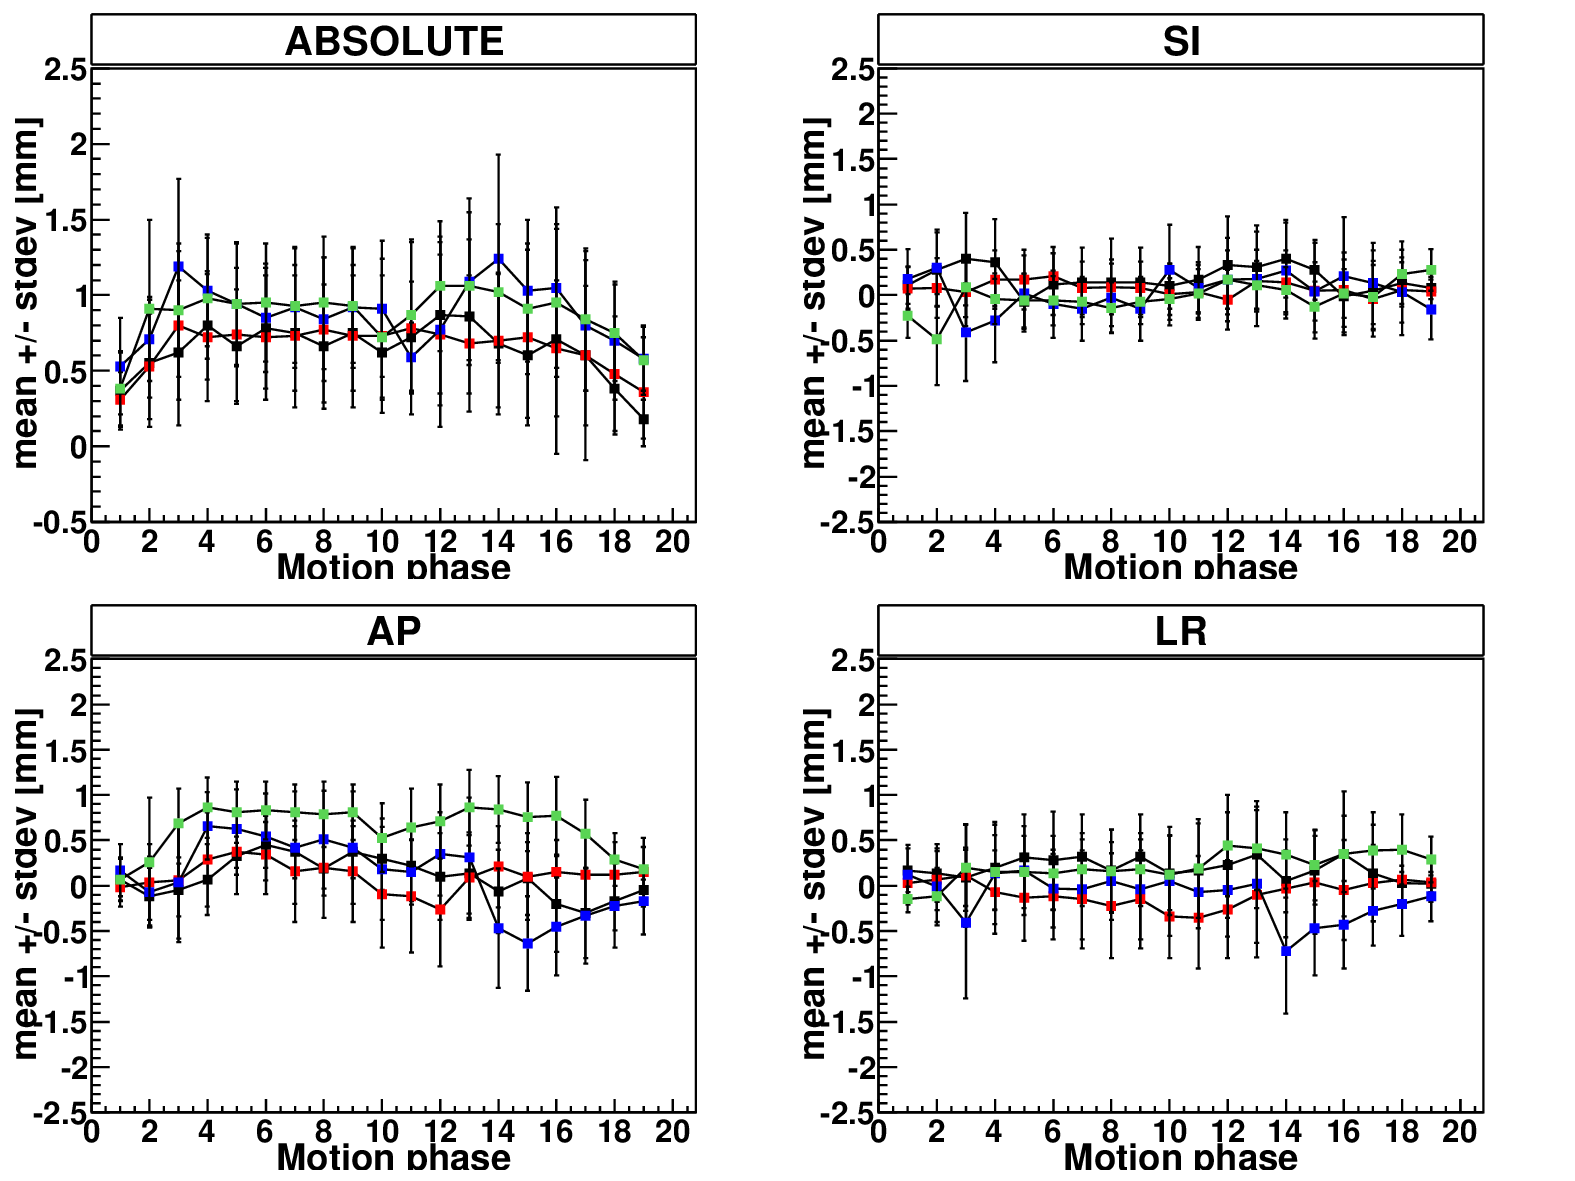
\includegraphics[scale=0.23]{Mayo_IPV_HB.png}
% % % \caption{Motion amplitude of IPV relative to the reference phase in each motion phase of heart beat. (pig 1: black, pig 2: red, pig 3: blue, 
% % % pig 4: green)}
% % % \end{center}
% % % \label{motion_hb_ipv}
% % % \end{figure}
% % % 
% % % \begin{figure}[H]
% % % \begin{center}
% % %  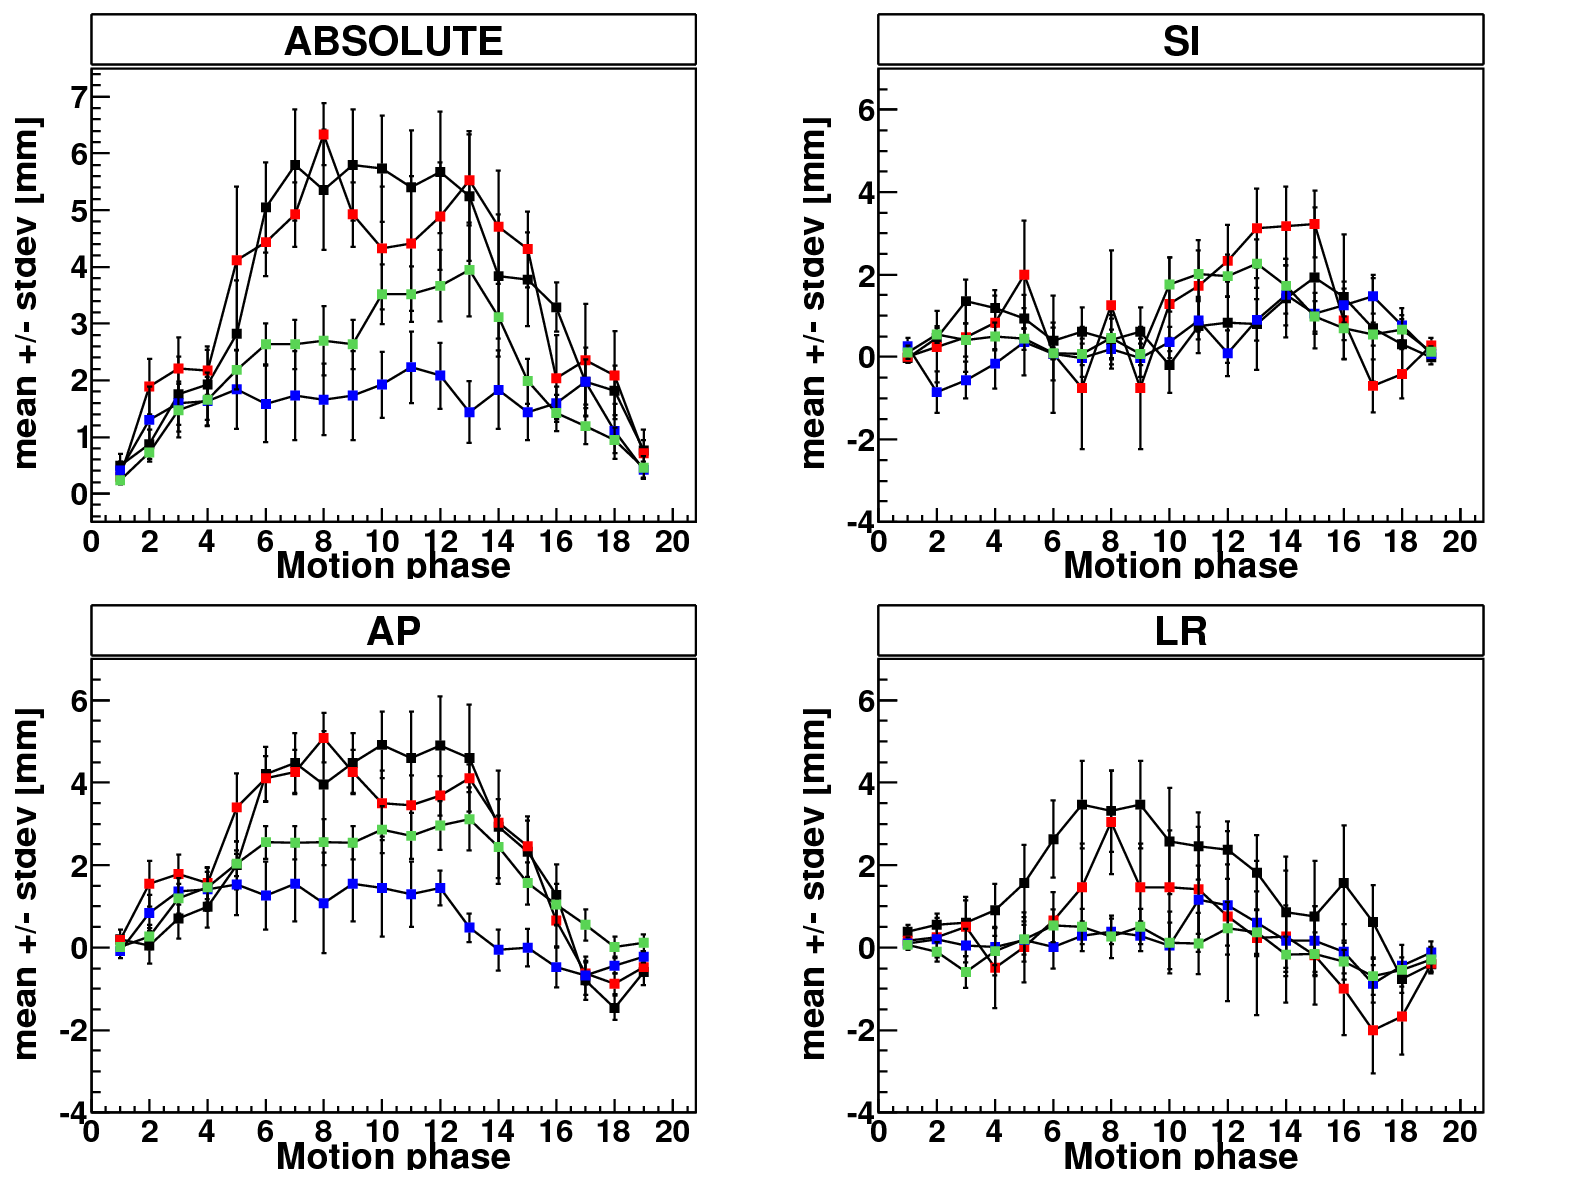
\includegraphics[scale=0.23]{Mayo_CTI_HB.png}
% % % \caption{Motion amplitude of CTI relative to the reference phase in each motion phase of heart beat. (pig 1: black, pig 2: red, pig 3: blue, 
% % % pig 4: green)}
% % % \end{center}
% % % \label{motion_hb_cti}
% % % \end{figure}
% % % 
% % % \newpage
% % % 
% % % \begin{figure}[H]
% % % \begin{center}
% % %  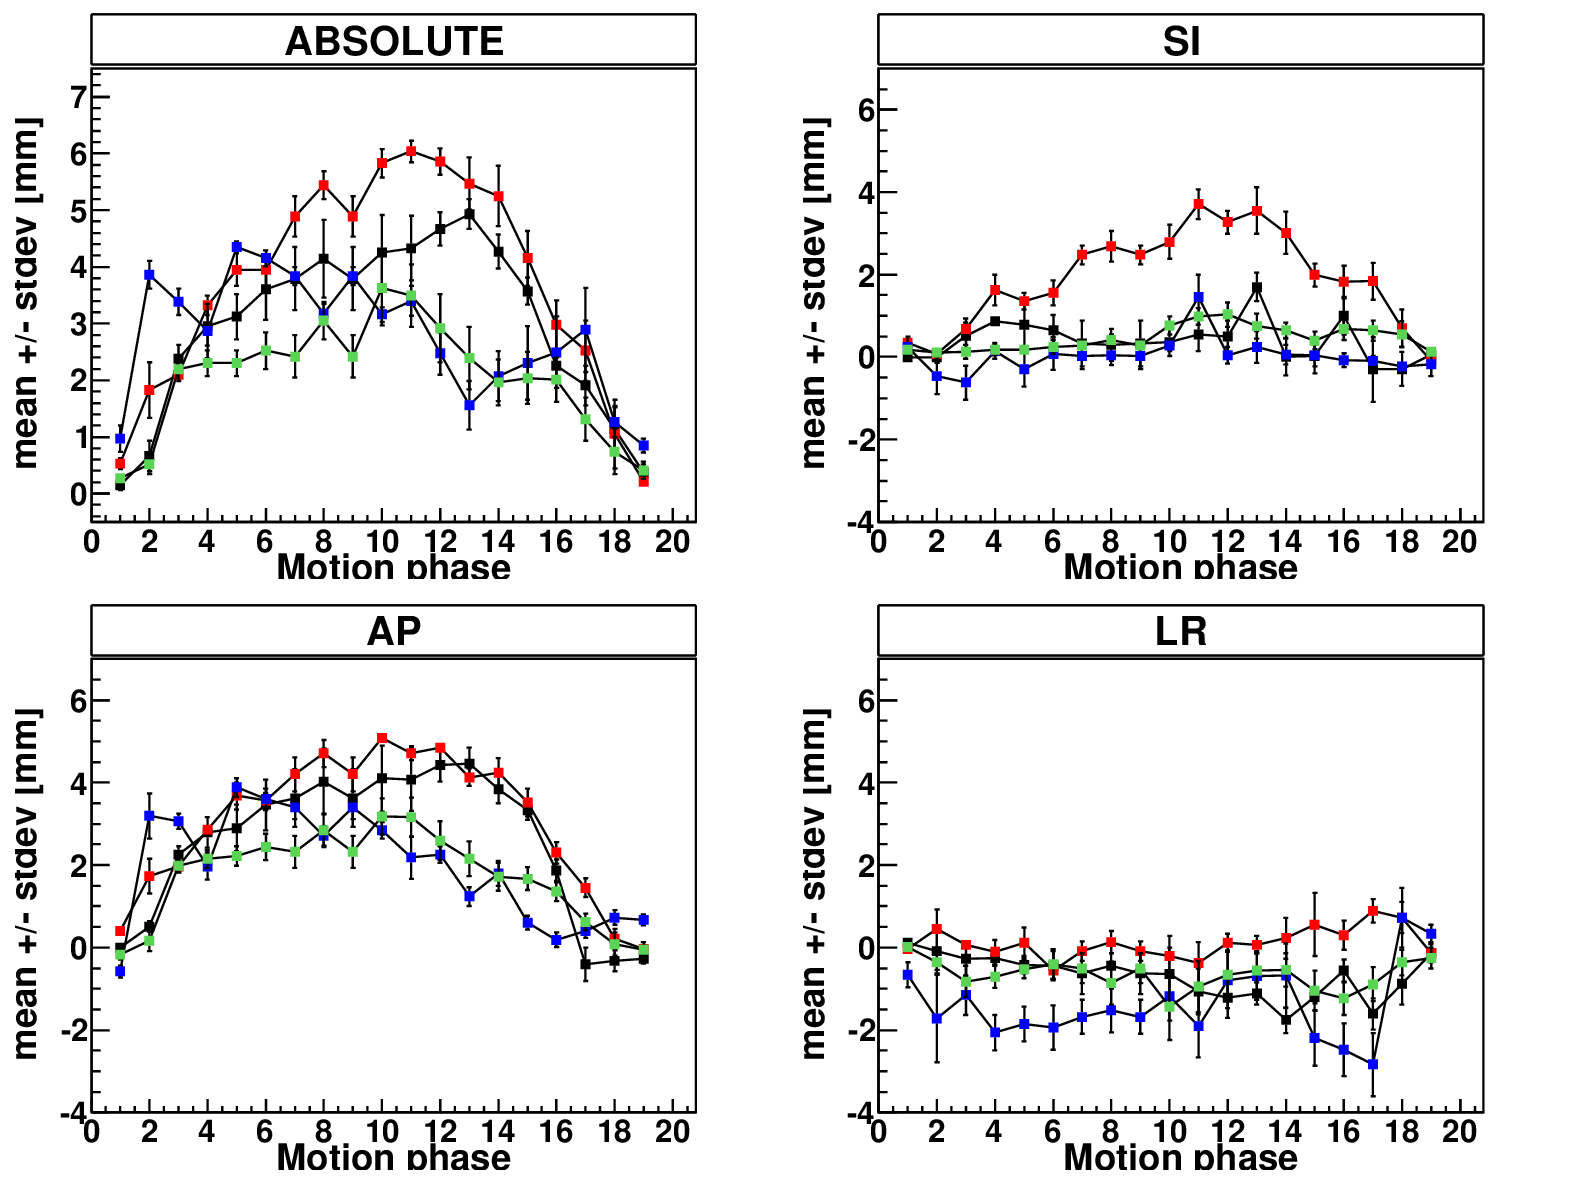
\includegraphics[scale=0.23]{Mayo_AV_HB.png}
% % % \caption{Motion amplitude of AV relative to the reference phase in each motion phase of heart beat. (pig 1: black, pig 2: red, pig 3: blue, 
% % % pig 4: green)}
% % % \end{center}
% % % \label{motion_hb_av}
% % % \end{figure}

%%%%%%%%%%%%%%%%%%%%%%%%%%%%%%%%%%%%%%%%%%%%%%%%%%%%%%%%%%%%%%%%%%%%%%%%%%%%%%%%%%%%%%%%%%%%%%%%%

\subsection{Interplay}

\subsubsection{Respiration}
\subsubsection{Heart beat}


\section{Discussion}

- grossere foki! -> auch hilfreich bei interplay!

- paper zu bewegung in schweineherzen?

\section{Summary}

\newpage

\section*{for APPENDIX}


\begin{table}[htbp]
  \centering
%      \scriptsize 
  \caption{PV: Mean and standard deviation of target motion in all phases of the heart beat, relative to the reference phase. The values are 
  taken from the contrast CTs of Pig 1.}
  \begin{tabular}{|c|c|c|c|c|}
    \hline\hline
    motion phase\rule{0pt}{2.6ex}\rule[-1.2ex]{0pt}{0pt} & ABS [mm] & SI [mm] & AP [mm] & LR [mm]\\
    \hline
01 &0.43 $\pm$ 0.23 &0.30 $\pm$ 0.25 &0.03 $\pm$ 0.13 &-0.10 $\pm$ 0.24 \\
02 &1.76 $\pm$ 0.52 &0.49 $\pm$ 0.28 &1.29 $\pm$ 0.33 &-0.79 $\pm$ 0.79 \\
03 &2.61 $\pm$ 0.30 &0.62 $\pm$ 0.39 &2.00 $\pm$ 0.49 &-1.16 $\pm$ 0.89 \\
04 &3.10 $\pm$ 0.28 &0.51 $\pm$ 0.41 &2.47 $\pm$ 0.68 &-1.27 $\pm$ 1.03 \\
05 &3.46 $\pm$ 0.39 &0.40 $\pm$ 0.57 &2.77 $\pm$ 0.90 &-1.42 $\pm$ 1.07 \\
06 &3.52 $\pm$ 0.59 &0.54 $\pm$ 0.64 &2.78 $\pm$ 1.09 &-1.31 $\pm$ 1.19 \\
07 &3.80 $\pm$ 0.77 &0.46 $\pm$ 0.86 &3.06 $\pm$ 1.32 &-1.32 $\pm$ 1.12 \\
08 &3.85 $\pm$ 0.98 &0.34 $\pm$ 1.04 &3.04 $\pm$ 1.60 &-1.13 $\pm$ 1.23 \\
09 &3.80 $\pm$ 0.77 &0.46 $\pm$ 0.86 &3.06 $\pm$ 1.32 &-1.32 $\pm$ 1.12 \\
10 &4.02 $\pm$ 1.09 &0.10 $\pm$ 1.42 &2.88 $\pm$ 1.85 &-1.01 $\pm$ 1.62 \\
11 &4.04 $\pm$ 1.14 &0.25 $\pm$ 1.57 &2.66 $\pm$ 2.09 &-1.11 $\pm$ 1.56 \\
12 &4.12 $\pm$ 1.13 &0.48 $\pm$ 1.68 &2.49 $\pm$ 2.25 &-1.16 $\pm$ 1.61 \\
13 &4.22 $\pm$ 1.07 &0.79 $\pm$ 1.56 &2.42 $\pm$ 2.22 &-1.40 $\pm$ 1.79 \\
14 &3.83 $\pm$ 0.88 &0.31 $\pm$ 1.76 &2.26 $\pm$ 1.58 &-1.77 $\pm$ 1.26 \\
15 &2.97 $\pm$ 0.72 &-0.00 $\pm$ 1.16 &2.02 $\pm$ 1.08 &-1.46 $\pm$ 0.77 \\
16 &1.94 $\pm$ 0.76 &-0.01 $\pm$ 0.75 &1.37 $\pm$ 0.79 &-1.01 $\pm$ 0.53 \\
17 &1.67 $\pm$ 0.55 &-0.60 $\pm$ 0.43 &1.12 $\pm$ 0.37 &-0.79 $\pm$ 0.72 \\
18 &1.17 $\pm$ 0.46 &-0.58 $\pm$ 0.30 &0.69 $\pm$ 0.39 &-0.34 $\pm$ 0.65 \\
19 &0.48 $\pm$ 0.23 &-0.36 $\pm$ 0.20 &0.05 $\pm$ 0.24 &-0.04 $\pm$ 0.23 \\
    \hline\hline
  \end{tabular}
  \label{tab:motion:PV:Pig1}
\end{table}

\newpage

\begin{table}[htbp]
  \centering
%      \scriptsize 
  \caption{CTI: Mean and standard deviation of target motion in all phases of the heart beat, relative to the reference phase. The values are 
  taken from the contrast CTs of Pig 1.}
  \begin{tabular}{|c|c|c|c|c|}
    \hline\hline
    motion phase\rule{0pt}{2.6ex}\rule[-1.2ex]{0pt}{0pt} & ABS [mm] & SI [mm] & AP [mm] & LR [mm]\\
    \hline
01 &0.49 $\pm$ 0.21 &-0.02 $\pm$ 0.13 &0.20 $\pm$ 0.23 &0.39 $\pm$ 0.16 \\
02 &0.87 $\pm$ 0.26 &0.46 $\pm$ 0.24 &0.04 $\pm$ 0.43 &0.55 $\pm$ 0.28 \\
03 &1.75 $\pm$ 0.66 &1.35 $\pm$ 0.53 &0.70 $\pm$ 0.48 &0.61 $\pm$ 0.54 \\
04 &1.92 $\pm$ 0.62 &1.18 $\pm$ 0.45 &0.99 $\pm$ 0.51 &0.91 $\pm$ 0.63 \\
05 &2.82 $\pm$ 0.94 &0.93 $\pm$ 0.57 &2.00 $\pm$ 0.58 &1.56 $\pm$ 0.93 \\
06 &5.05 $\pm$ 0.80 &0.39 $\pm$ 0.45 &4.20 $\pm$ 0.66 &2.63 $\pm$ 0.93 \\
07 &5.79 $\pm$ 0.98 &0.62 $\pm$ 0.58 &4.48 $\pm$ 0.73 &3.47 $\pm$ 1.06 \\
08 &5.36 $\pm$ 1.06 &0.42 $\pm$ 0.60 &3.95 $\pm$ 1.31 &3.31 $\pm$ 0.99 \\
09 &5.79 $\pm$ 0.98 &0.62 $\pm$ 0.58 &4.48 $\pm$ 0.73 &3.47 $\pm$ 1.06 \\
10 &5.73 $\pm$ 0.94 &-0.20 $\pm$ 0.66 &4.92 $\pm$ 0.81 &2.58 $\pm$ 1.29 \\
11 &5.40 $\pm$ 1.01 &0.75 $\pm$ 0.65 &4.60 $\pm$ 1.13 &2.46 $\pm$ 0.82 \\
12 &5.67 $\pm$ 1.07 &0.84 $\pm$ 0.98 &4.90 $\pm$ 1.20 &2.37 $\pm$ 0.70 \\
13 &5.25 $\pm$ 1.14 &0.80 $\pm$ 1.11 &4.60 $\pm$ 1.30 &1.82 $\pm$ 0.91 \\
14 &3.83 $\pm$ 1.10 &1.43 $\pm$ 0.95 &2.92 $\pm$ 1.38 &0.86 $\pm$ 1.35 \\
15 &3.78 $\pm$ 0.83 &1.92 $\pm$ 1.71 &2.32 $\pm$ 0.76 &0.76 $\pm$ 1.35 \\
16 &3.29 $\pm$ 0.44 &1.46 $\pm$ 1.52 &1.28 $\pm$ 0.74 &1.56 $\pm$ 1.40 \\
17 &1.97 $\pm$ 0.60 &0.70 $\pm$ 1.30 &-0.80 $\pm$ 0.47 &0.62 $\pm$ 0.90 \\
18 &1.82 $\pm$ 0.43 &0.31 $\pm$ 0.71 &-1.46 $\pm$ 0.30 &-0.76 $\pm$ 0.33 \\
19 &0.76 $\pm$ 0.37 &-0.01 $\pm$ 0.17 &-0.60 $\pm$ 0.32 &-0.40 $\pm$ 0.23 \\
    \hline\hline
  \end{tabular}
  \label{tab:motion:CTI:Pig1}
\end{table}

\newpage

\begin{table}[htbp]
  \centering
  \caption{AV node: Mean and standard deviation of target motion in all phases of the heart beat, relative to the reference phase. The values are 
  taken from the contrast CTs of Pig 1.}
  \begin{tabular}{|c|c|c|c|c|}
    \hline\hline
    motion phase\rule{0pt}{2.6ex}\rule[-1.2ex]{0pt}{0pt} & ABS [mm] & SI [mm] & AP [mm] & LR [mm]\\
    \hline
01 &0.15 $\pm$ 0.09 &-0.01 $\pm$ 0.06 &-0.01 $\pm$ 0.04 &0.12 $\pm$ 0.10 \\
02 &0.66 $\pm$ 0.27 &-0.01 $\pm$ 0.14 &0.51 $\pm$ 0.12 &-0.08 $\pm$ 0.46 \\
03 &2.38 $\pm$ 0.24 &0.52 $\pm$ 0.31 &2.25 $\pm$ 0.21 &-0.28 $\pm$ 0.41 \\
04 &2.95 $\pm$ 0.34 &0.87 $\pm$ 0.11 &2.80 $\pm$ 0.37 &-0.25 $\pm$ 0.18 \\
05 &3.12 $\pm$ 0.40 &0.79 $\pm$ 0.60 &2.90 $\pm$ 0.56 &-0.42 $\pm$ 0.21 \\
06 &3.60 $\pm$ 0.53 &0.64 $\pm$ 0.38 &3.46 $\pm$ 0.62 &-0.44 $\pm$ 0.36 \\
07 &3.79 $\pm$ 0.56 &0.33 $\pm$ 0.55 &3.62 $\pm$ 0.70 &-0.63 $\pm$ 0.50 \\
08 &4.14 $\pm$ 0.69 &0.29 $\pm$ 0.39 &4.03 $\pm$ 0.80 &-0.44 $\pm$ 0.56 \\
09 &3.79 $\pm$ 0.56 &0.33 $\pm$ 0.55 &3.62 $\pm$ 0.70 &-0.63 $\pm$ 0.50 \\
10 &4.25 $\pm$ 0.66 &0.36 $\pm$ 0.33 &4.10 $\pm$ 0.80 &-0.64 $\pm$ 0.63 \\
11 &4.33 $\pm$ 0.57 &0.54 $\pm$ 0.39 &4.08 $\pm$ 0.76 &-1.06 $\pm$ 0.56 \\
12 &4.67 $\pm$ 0.29 &0.49 $\pm$ 0.40 &4.43 $\pm$ 0.41 &-1.21 $\pm$ 0.50 \\
13 &4.93 $\pm$ 0.26 &1.70 $\pm$ 0.35 &4.46 $\pm$ 0.39 &-1.11 $\pm$ 0.27 \\
14 &4.27 $\pm$ 0.30 &0.00 $\pm$ 0.44 &3.84 $\pm$ 0.34 &-1.76 $\pm$ 0.31 \\
15 &3.57 $\pm$ 0.24 &0.03 $\pm$ 0.42 &3.33 $\pm$ 0.23 &-1.20 $\pm$ 0.15 \\
16 &2.25 $\pm$ 0.21 &1.00 $\pm$ 0.46 &1.86 $\pm$ 0.28 &-0.56 $\pm$ 0.27 \\
17 &1.91 $\pm$ 0.35 &-0.30 $\pm$ 0.78 &-0.41 $\pm$ 0.40 &-1.61 $\pm$ 0.38 \\
18 &1.14 $\pm$ 0.40 &-0.29 $\pm$ 0.41 &-0.32 $\pm$ 0.25 &-0.88 $\pm$ 0.51 \\
19 &0.37 $\pm$ 0.15 &0.06 $\pm$ 0.06 &-0.27 $\pm$ 0.12 &-0.14 $\pm$ 0.22 \\
    \hline\hline
  \end{tabular}
  \label{tab:motion:AV:Pig1}
\end{table}

\newpage


\begin{table}[htbp]
  \centering
  \caption{PV: Mean and standard deviation of target motion in all phases of the heart beat, relative to the reference phase. The values are 
  taken from the contrast CTs of Pig 2.}
  \begin{tabular}{|c|c|c|c|c|}
    \hline\hline
    motion phase\rule{0pt}{2.6ex}\rule[-1.2ex]{0pt}{0pt} & ABS [mm] & SI [mm] & AP [mm] & LR [mm]\\
    \hline
01 &0.37 $\pm$ 0.25 &0.02 $\pm$ 0.27 &0.14 $\pm$ 0.20 &-0.10 $\pm$ 0.24 \\
02 &1.16 $\pm$ 0.69 &0.40 $\pm$ 0.42 &0.78 $\pm$ 0.58 &-0.43 $\pm$ 0.60 \\
03 &2.06 $\pm$ 0.57 &0.73 $\pm$ 0.47 &1.61 $\pm$ 0.63 &-0.61 $\pm$ 0.69 \\
04 &2.26 $\pm$ 0.64 &0.79 $\pm$ 0.47 &1.74 $\pm$ 0.75 &-0.77 $\pm$ 0.69 \\
05 &2.50 $\pm$ 0.66 &1.09 $\pm$ 0.65 &1.82 $\pm$ 0.80 &-0.61 $\pm$ 0.89 \\
06 &2.71 $\pm$ 0.96 &1.26 $\pm$ 0.85 &1.89 $\pm$ 1.04 &-0.51 $\pm$ 1.02 \\
07 &3.02 $\pm$ 1.11 &1.33 $\pm$ 0.95 &2.14 $\pm$ 1.35 &-0.67 $\pm$ 0.91 \\
08 &3.09 $\pm$ 1.22 &1.20 $\pm$ 0.96 &2.18 $\pm$ 1.50 &-0.47 $\pm$ 1.22 \\
09 &3.02 $\pm$ 1.11 &1.33 $\pm$ 0.95 &2.14 $\pm$ 1.35 &-0.67 $\pm$ 0.91 \\
10 &3.30 $\pm$ 1.12 &1.21 $\pm$ 1.24 &1.81 $\pm$ 1.72 &-0.64 $\pm$ 1.57 \\
11 &3.24 $\pm$ 1.14 &1.33 $\pm$ 1.33 &1.60 $\pm$ 1.68 &-0.68 $\pm$ 1.57 \\
12 &3.71 $\pm$ 1.55 &1.50 $\pm$ 1.46 &2.08 $\pm$ 2.05 &-0.81 $\pm$ 1.61 \\
13 &3.37 $\pm$ 1.23 &1.67 $\pm$ 1.41 &1.62 $\pm$ 1.58 &-0.92 $\pm$ 1.46 \\
14 &2.92 $\pm$ 1.11 &1.55 $\pm$ 1.26 &1.42 $\pm$ 1.25 &-0.97 $\pm$ 1.12 \\
15 &2.19 $\pm$ 1.00 &1.12 $\pm$ 1.00 &1.27 $\pm$ 0.87 &-0.70 $\pm$ 0.83 \\
16 &1.80 $\pm$ 0.70 &0.10 $\pm$ 0.61 &0.87 $\pm$ 0.86 &-1.01 $\pm$ 0.90 \\
17 &1.52 $\pm$ 0.69 &-0.19 $\pm$ 0.61 &0.72 $\pm$ 0.71 &-0.86 $\pm$ 0.79 \\
18 &1.11 $\pm$ 0.57 &-0.23 $\pm$ 0.58 &0.21 $\pm$ 0.65 &-0.50 $\pm$ 0.66 \\
19 &0.39 $\pm$ 0.25 &-0.04 $\pm$ 0.32 &0.10 $\pm$ 0.21 &-0.03 $\pm$ 0.23 \\
    \hline\hline
  \end{tabular}
  \label{tab:motion:PV:Pig2}
\end{table}

\newpage

\begin{table}[htbp]
  \centering
  \caption{CTI: Mean and standard deviation of target motion in all phases of the heart beat, relative to the reference phase. The values are 
  taken from the contrast CTs of Pig 2.}
  \begin{tabular}{|c|c|c|c|c|}
    \hline\hline
    motion phase\rule{0pt}{2.6ex}\rule[-1.2ex]{0pt}{0pt} & ABS [mm] & SI [mm] & AP [mm] & LR [mm]\\
    \hline
01 &0.29 $\pm$ 0.13 &-0.00 $\pm$ 0.13 &0.19 $\pm$ 0.11 &0.16 $\pm$ 0.11 \\
02 &1.89 $\pm$ 0.49 &0.25 $\pm$ 0.87 &1.55 $\pm$ 0.56 &0.25 $\pm$ 0.48 \\
03 &2.21 $\pm$ 0.55 &0.48 $\pm$ 0.85 &1.79 $\pm$ 0.46 &0.51 $\pm$ 0.72 \\
04 &2.17 $\pm$ 0.43 &0.84 $\pm$ 0.65 &1.56 $\pm$ 0.39 &-0.49 $\pm$ 0.98 \\
05 &4.12 $\pm$ 1.29 &2.00 $\pm$ 1.31 &3.40 $\pm$ 0.82 &0.01 $\pm$ 0.85 \\
06 &4.43 $\pm$ 0.60 &0.07 $\pm$ 1.42 &4.10 $\pm$ 0.55 &0.66 $\pm$ 0.68 \\
07 &4.92 $\pm$ 0.57 &-0.75 $\pm$ 1.49 &4.26 $\pm$ 0.54 &1.47 $\pm$ 1.06 \\
08 &6.34 $\pm$ 0.54 &1.26 $\pm$ 1.32 &5.09 $\pm$ 0.60 &3.04 $\pm$ 1.25 \\
09 &4.92 $\pm$ 0.57 &-0.75 $\pm$ 1.49 &4.26 $\pm$ 0.54 &1.47 $\pm$ 1.06 \\
10 &4.33 $\pm$ 1.08 &1.28 $\pm$ 1.14 &3.50 $\pm$ 0.80 &1.46 $\pm$ 1.38 \\
11 &4.41 $\pm$ 1.19 &1.72 $\pm$ 1.11 &3.45 $\pm$ 0.72 &1.41 $\pm$ 1.51 \\
12 &4.89 $\pm$ 0.95 &2.34 $\pm$ 0.86 &3.68 $\pm$ 0.48 &0.76 $\pm$ 2.06 \\
13 &5.53 $\pm$ 0.80 &3.12 $\pm$ 0.96 &4.11 $\pm$ 0.34 &0.23 $\pm$ 1.87 \\
14 &4.70 $\pm$ 1.00 &3.17 $\pm$ 0.96 &3.03 $\pm$ 0.57 &0.26 $\pm$ 1.60 \\
15 &4.31 $\pm$ 0.67 &3.22 $\pm$ 0.81 &2.45 $\pm$ 0.73 &-0.19 $\pm$ 1.20 \\
16 &2.03 $\pm$ 0.77 &0.89 $\pm$ 0.94 &0.65 $\pm$ 0.62 &-1.00 $\pm$ 1.12 \\
17 &2.35 $\pm$ 0.99 &-0.70 $\pm$ 0.64 &-0.63 $\pm$ 0.27 &-2.01 $\pm$ 1.04 \\
18 &2.09 $\pm$ 0.78 &-0.41 $\pm$ 0.60 &-0.88 $\pm$ 0.25 &-1.67 $\pm$ 0.92 \\
19 &0.71 $\pm$ 0.23 &0.28 $\pm$ 0.18 &-0.48 $\pm$ 0.18 &-0.39 $\pm$ 0.19 \\
    \hline\hline
  \end{tabular}
  \label{tab:motion:CTI:Pig2}
\end{table}

\newpage

\begin{table}[htbp]
  \centering
  \caption{AV node: Mean and standard deviation of target motion in all phases of the heart beat, relative to the reference phase. The values are 
  taken from the contrast CTs of Pig 2.}
  \begin{tabular}{|c|c|c|c|c|}
    \hline\hline
    motion phase\rule{0pt}{2.6ex}\rule[-1.2ex]{0pt}{0pt} & ABS [mm] & SI [mm] & AP [mm] & LR [mm]\\
    \hline
01 &0.53 $\pm$ 0.10 &0.34 $\pm$ 0.09 &0.40 $\pm$ 0.07 &-0.04 $\pm$ 0.05 \\
02 &1.83 $\pm$ 0.49 &0.08 $\pm$ 0.10 &1.73 $\pm$ 0.42 &0.46 $\pm$ 0.46 \\
03 &2.10 $\pm$ 0.08 &0.68 $\pm$ 0.25 &1.97 $\pm$ 0.14 &0.06 $\pm$ 0.09 \\
04 &3.32 $\pm$ 0.17 &1.62 $\pm$ 0.37 &2.86 $\pm$ 0.09 &-0.11 $\pm$ 0.30 \\
05 &3.95 $\pm$ 0.29 &1.35 $\pm$ 0.20 &3.68 $\pm$ 0.33 &0.12 $\pm$ 0.37 \\
06 &3.94 $\pm$ 0.28 &1.56 $\pm$ 0.30 &3.56 $\pm$ 0.20 &-0.56 $\pm$ 0.20 \\
07 &4.89 $\pm$ 0.36 &2.48 $\pm$ 0.23 &4.20 $\pm$ 0.41 &-0.09 $\pm$ 0.24 \\
08 &5.44 $\pm$ 0.25 &2.68 $\pm$ 0.37 &4.71 $\pm$ 0.33 &0.14 $\pm$ 0.27 \\
09 &4.89 $\pm$ 0.36 &2.48 $\pm$ 0.23 &4.20 $\pm$ 0.41 &-0.09 $\pm$ 0.24 \\
10 &5.83 $\pm$ 0.25 &2.79 $\pm$ 0.41 &5.08 $\pm$ 0.11 &-0.21 $\pm$ 0.49 \\
11 &6.04 $\pm$ 0.19 &3.71 $\pm$ 0.36 &4.71 $\pm$ 0.17 &-0.38 $\pm$ 0.51 \\
12 &5.86 $\pm$ 0.23 &3.27 $\pm$ 0.28 &4.85 $\pm$ 0.11 &0.12 $\pm$ 0.22 \\
13 &5.47 $\pm$ 0.46 &3.55 $\pm$ 0.56 &4.13 $\pm$ 0.21 &0.07 $\pm$ 0.21 \\
14 &5.25 $\pm$ 0.53 &3.01 $\pm$ 0.51 &4.25 $\pm$ 0.35 &0.23 $\pm$ 0.50 \\
15 &4.15 $\pm$ 0.48 &1.99 $\pm$ 0.28 &3.52 $\pm$ 0.34 &0.56 $\pm$ 0.76 \\
16 &2.98 $\pm$ 0.43 &1.82 $\pm$ 0.40 &2.30 $\pm$ 0.26 &0.30 $\pm$ 0.36 \\
17 &2.52 $\pm$ 0.53 &1.84 $\pm$ 0.45 &1.45 $\pm$ 0.23 &0.89 $\pm$ 0.28 \\
18 &1.05 $\pm$ 0.61 &0.70 $\pm$ 0.46 &0.21 $\pm$ 0.24 &0.73 $\pm$ 0.38 \\
19 &0.21 $\pm$ 0.06 &-0.10 $\pm$ 0.06 &-0.03 $\pm$ 0.08 &-0.14 $\pm$ 0.09 \\
    \hline\hline
  \end{tabular}
  \label{tab:motion:AV:Pig2}
\end{table}

\newpage


\begin{table}[htbp]
  \centering
  \caption{PV: Mean and standard deviation of target motion in all phases of the heart beat, relative to the reference phase. The values are 
  taken from the contrast CTs of Pig 3.}
  \begin{tabular}{|c|c|c|c|c|}
    \hline\hline
    motion phase\rule{0pt}{2.6ex}\rule[-1.2ex]{0pt}{0pt} & ABS [mm] & SI [mm] & AP [mm] & LR [mm]\\
    \hline
01 &0.59 $\pm$ 0.27 &0.05 $\pm$ 0.22 &-0.07 $\pm$ 0.42 &0.25 $\pm$ 0.35 \\
02 &1.39 $\pm$ 0.85 &-0.21 $\pm$ 0.41 &1.13 $\pm$ 0.85 &0.46 $\pm$ 0.50 \\
03 &2.09 $\pm$ 0.80 &-0.15 $\pm$ 0.48 &1.67 $\pm$ 0.70 &0.69 $\pm$ 1.01 \\
04 &2.17 $\pm$ 0.85 &-0.27 $\pm$ 0.50 &1.64 $\pm$ 0.73 &0.81 $\pm$ 1.11 \\
05 &2.21 $\pm$ 0.89 &-0.41 $\pm$ 0.57 &1.94 $\pm$ 0.81 &0.41 $\pm$ 0.79 \\
06 &2.39 $\pm$ 0.89 &-0.48 $\pm$ 0.58 &2.10 $\pm$ 0.80 &0.42 $\pm$ 0.85 \\
07 &2.36 $\pm$ 0.91 &-0.48 $\pm$ 0.65 &2.00 $\pm$ 0.83 &0.44 $\pm$ 0.92 \\
08 &2.23 $\pm$ 0.97 &-0.55 $\pm$ 0.67 &1.77 $\pm$ 0.89 &0.47 $\pm$ 1.01 \\
09 &2.36 $\pm$ 0.91 &-0.48 $\pm$ 0.65 &2.00 $\pm$ 0.83 &0.44 $\pm$ 0.92 \\
10 &1.79 $\pm$ 0.74 &-0.19 $\pm$ 0.54 &1.29 $\pm$ 0.77 &0.32 $\pm$ 1.03 \\
11 &1.61 $\pm$ 0.76 &0.06 $\pm$ 0.56 &0.92 $\pm$ 0.85 &0.16 $\pm$ 1.12 \\
12 &1.54 $\pm$ 0.57 &-0.13 $\pm$ 0.43 &0.53 $\pm$ 1.03 &-0.17 $\pm$ 1.07 \\
13 &1.21 $\pm$ 0.52 &0.01 $\pm$ 0.41 &0.31 $\pm$ 0.82 &-0.44 $\pm$ 0.77 \\
14 &1.53 $\pm$ 0.59 &0.09 $\pm$ 0.45 &-0.52 $\pm$ 1.31 &-0.42 $\pm$ 0.58 \\
15 &1.38 $\pm$ 0.59 &-0.13 $\pm$ 0.49 &-0.52 $\pm$ 1.09 &-0.59 $\pm$ 0.46 \\
16 &1.58 $\pm$ 0.77 &-0.16 $\pm$ 0.59 &-0.80 $\pm$ 1.21 &-0.56 $\pm$ 0.53 \\
17 &1.76 $\pm$ 1.05 &-0.13 $\pm$ 0.76 &-1.08 $\pm$ 1.35 &-0.54 $\pm$ 0.60 \\
18 &1.65 $\pm$ 0.98 &-0.11 $\pm$ 0.81 &-1.12 $\pm$ 1.15 &-0.25 $\pm$ 0.59 \\
19 &0.63 $\pm$ 0.43 &0.03 $\pm$ 0.36 &-0.22 $\pm$ 0.33 &-0.29 $\pm$ 0.47 \\
    \hline\hline
  \end{tabular}
  \label{tab:motion:PV:Pig3}
\end{table}

\newpage

\begin{table}[htbp]
  \centering
  \caption{CTI: Mean and standard deviation of target motion in all phases of the heart beat, relative to the reference phase. The values are 
  taken from the contrast CTs of Pig 3.}
  \begin{tabular}{|c|c|c|c|c|}
    \hline\hline
    motion phase\rule{0pt}{2.6ex}\rule[-1.2ex]{0pt}{0pt} & ABS [mm] & SI [mm] & AP [mm] & LR [mm]\\
    \hline
01 &0.40 $\pm$ 0.16 &0.26 $\pm$ 0.21 &-0.08 $\pm$ 0.18 &0.10 $\pm$ 0.15 \\
02 &1.30 $\pm$ 0.59 &-0.85 $\pm$ 0.50 &0.84 $\pm$ 0.43 &0.20 $\pm$ 0.38 \\
03 &1.59 $\pm$ 0.38 &-0.56 $\pm$ 0.45 &1.37 $\pm$ 0.32 &0.05 $\pm$ 0.40 \\
04 &1.63 $\pm$ 0.43 &-0.16 $\pm$ 0.60 &1.41 $\pm$ 0.52 &0.02 $\pm$ 0.45 \\
05 &1.84 $\pm$ 0.70 &0.37 $\pm$ 0.82 &1.53 $\pm$ 0.74 &0.19 $\pm$ 0.36 \\
06 &1.58 $\pm$ 0.67 &0.08 $\pm$ 0.64 &1.26 $\pm$ 0.82 &0.02 $\pm$ 0.53 \\
07 &1.73 $\pm$ 0.78 &-0.02 $\pm$ 0.46 &1.54 $\pm$ 0.91 &0.28 $\pm$ 0.36 \\
08 &1.66 $\pm$ 0.63 &0.19 $\pm$ 0.47 &1.08 $\pm$ 1.22 &0.39 $\pm$ 0.31 \\
09 &1.73 $\pm$ 0.78 &-0.02 $\pm$ 0.46 &1.54 $\pm$ 0.91 &0.28 $\pm$ 0.36 \\
10 &1.92 $\pm$ 0.58 &0.36 $\pm$ 0.38 &1.44 $\pm$ 1.17 &0.04 $\pm$ 0.56 \\
11 &2.23 $\pm$ 0.63 &0.89 $\pm$ 0.46 &1.30 $\pm$ 0.79 &1.16 $\pm$ 0.83 \\
12 &2.08 $\pm$ 0.58 &0.09 $\pm$ 0.55 &1.45 $\pm$ 0.42 &1.03 $\pm$ 0.99 \\
13 &1.44 $\pm$ 0.55 &0.90 $\pm$ 0.51 &0.48 $\pm$ 0.35 &0.60 $\pm$ 0.76 \\
14 &1.83 $\pm$ 0.69 &1.50 $\pm$ 0.73 &-0.06 $\pm$ 0.49 &0.16 $\pm$ 0.86 \\
15 &1.43 $\pm$ 0.49 &1.06 $\pm$ 0.49 &-0.00 $\pm$ 0.46 &0.17 $\pm$ 0.83 \\
16 &1.60 $\pm$ 0.29 &1.25 $\pm$ 0.41 &-0.48 $\pm$ 0.48 &-0.10 $\pm$ 0.67 \\
17 &1.97 $\pm$ 0.40 &1.48 $\pm$ 0.43 &-0.68 $\pm$ 0.46 &-0.88 $\pm$ 0.45 \\
18 &1.10 $\pm$ 0.48 &0.77 $\pm$ 0.41 &-0.44 $\pm$ 0.19 &-0.44 $\pm$ 0.51 \\
19 &0.42 $\pm$ 0.14 &0.08 $\pm$ 0.18 &-0.22 $\pm$ 0.14 &-0.12 $\pm$ 0.27 \\
    \hline\hline
  \end{tabular}
  \label{tab:motion:CTI:Pig3}
\end{table}

\newpage

\begin{table}[htbp]
  \centering
  \caption{AV node: Mean and standard deviation of target motion in all phases of the heart beat, relative to the reference phase. The values are 
  taken from the contrast CTs of Pig 3.}
  \begin{tabular}{|c|c|c|c|c|}
    \hline\hline
    motion phase\rule{0pt}{2.6ex}\rule[-1.2ex]{0pt}{0pt} & ABS [mm] & SI [mm] & AP [mm] & LR [mm]\\
    \hline
01 &0.97 $\pm$ 0.23 &0.25 $\pm$ 0.24 &-0.58 $\pm$ 0.14 &-0.66 $\pm$ 0.30 \\
02 &3.86 $\pm$ 0.24 &-0.46 $\pm$ 0.45 &3.19 $\pm$ 0.54 &-1.72 $\pm$ 1.06 \\
03 &3.38 $\pm$ 0.23 &-0.62 $\pm$ 0.41 &3.06 $\pm$ 0.18 &-1.15 $\pm$ 0.48 \\
04 &2.87 $\pm$ 0.48 &0.15 $\pm$ 0.20 &1.97 $\pm$ 0.33 &-2.06 $\pm$ 0.43 \\
05 &4.35 $\pm$ 0.10 &-0.30 $\pm$ 0.41 &3.88 $\pm$ 0.23 &-1.85 $\pm$ 0.42 \\
06 &4.15 $\pm$ 0.14 &0.08 $\pm$ 0.40 &3.60 $\pm$ 0.26 &-1.94 $\pm$ 0.54 \\
07 &3.84 $\pm$ 0.16 &0.02 $\pm$ 0.31 &3.40 $\pm$ 0.29 &-1.68 $\pm$ 0.41 \\
08 &3.17 $\pm$ 0.17 &0.04 $\pm$ 0.24 &2.71 $\pm$ 0.24 &-1.51 $\pm$ 0.55 \\
09 &3.84 $\pm$ 0.16 &0.02 $\pm$ 0.31 &3.40 $\pm$ 0.29 &-1.68 $\pm$ 0.41 \\
10 &3.16 $\pm$ 0.13 &0.28 $\pm$ 0.13 &2.85 $\pm$ 0.20 &-1.18 $\pm$ 0.59 \\
11 &3.40 $\pm$ 0.26 &1.46 $\pm$ 0.54 &2.18 $\pm$ 0.52 &-1.91 $\pm$ 0.76 \\
12 &2.47 $\pm$ 0.37 &0.04 $\pm$ 0.20 &2.26 $\pm$ 0.20 &-0.79 $\pm$ 0.68 \\
13 &1.56 $\pm$ 0.43 &0.24 $\pm$ 0.39 &1.24 $\pm$ 0.23 &-0.70 $\pm$ 0.57 \\
14 &2.07 $\pm$ 0.44 &0.06 $\pm$ 0.23 &1.80 $\pm$ 0.30 &-0.68 $\pm$ 0.78 \\
15 &2.30 $\pm$ 0.65 &0.04 $\pm$ 0.26 &0.60 $\pm$ 0.17 &-2.20 $\pm$ 0.66 \\
16 &2.49 $\pm$ 0.63 &-0.07 $\pm$ 0.17 &0.19 $\pm$ 0.18 &-2.47 $\pm$ 0.64 \\
17 &2.89 $\pm$ 0.74 &-0.10 $\pm$ 0.13 &0.41 $\pm$ 0.17 &-2.84 $\pm$ 0.76 \\
18 &1.26 $\pm$ 0.26 &-0.22 $\pm$ 0.11 &0.73 $\pm$ 0.17 &0.72 $\pm$ 0.72 \\
19 &0.85 $\pm$ 0.12 &-0.18 $\pm$ 0.28 &0.67 $\pm$ 0.14 &0.34 $\pm$ 0.21 \\
    \hline\hline
  \end{tabular}
  \label{tab:motion:AV:Pig3}
\end{table}

\newpage


\begin{table}[htbp]
  \centering
  \caption{PV: Mean and standard deviation of target motion in all phases of the heart beat, relative to the reference phase. The values are 
  taken from the contrast CTs of Pig 4.}
  \begin{tabular}{|c|c|c|c|c|}
    \hline\hline
    motion phase\rule{0pt}{2.6ex}\rule[-1.2ex]{0pt}{0pt} & ABS [mm] & SI [mm] & AP [mm] & LR [mm]\\
    \hline
01 &0.52 $\pm$ 0.31 &0.22 $\pm$ 0.31 &0.29 $\pm$ 0.27 &-0.07 $\pm$ 0.22 \\
02 &1.72 $\pm$ 0.39 &0.09 $\pm$ 0.27 &1.56 $\pm$ 0.32 &-0.44 $\pm$ 0.53 \\
03 &2.21 $\pm$ 0.28 &0.07 $\pm$ 0.29 &1.96 $\pm$ 0.22 &-0.73 $\pm$ 0.66 \\
04 &2.39 $\pm$ 0.23 &0.22 $\pm$ 0.32 &2.14 $\pm$ 0.33 &-0.63 $\pm$ 0.75 \\
05 &2.48 $\pm$ 0.38 &0.14 $\pm$ 0.34 &2.24 $\pm$ 0.53 &-0.37 $\pm$ 0.86 \\
06 &2.48 $\pm$ 0.56 &0.14 $\pm$ 0.33 &2.24 $\pm$ 0.71 &-0.23 $\pm$ 0.86 \\
07 &2.38 $\pm$ 0.68 &0.29 $\pm$ 0.33 &2.12 $\pm$ 0.86 &-0.25 $\pm$ 0.80 \\
08 &2.34 $\pm$ 0.80 &0.41 $\pm$ 0.38 &1.99 $\pm$ 1.00 &-0.30 $\pm$ 0.86 \\
09 &2.38 $\pm$ 0.68 &0.29 $\pm$ 0.33 &2.12 $\pm$ 0.86 &-0.25 $\pm$ 0.80 \\
10 &3.05 $\pm$ 1.06 &0.70 $\pm$ 0.59 &2.45 $\pm$ 1.36 &-0.59 $\pm$ 1.19 \\
11 &3.13 $\pm$ 1.03 &0.81 $\pm$ 0.67 &2.64 $\pm$ 1.17 &-0.49 $\pm$ 1.09 \\
12 &2.82 $\pm$ 0.80 &0.80 $\pm$ 0.63 &2.44 $\pm$ 0.84 &-0.37 $\pm$ 0.87 \\
13 &2.38 $\pm$ 0.74 &0.56 $\pm$ 0.62 &2.19 $\pm$ 0.68 &-0.08 $\pm$ 0.51 \\
14 &2.17 $\pm$ 0.63 &0.45 $\pm$ 0.52 &2.02 $\pm$ 0.58 &0.13 $\pm$ 0.48 \\
15 &2.05 $\pm$ 0.45 &0.22 $\pm$ 0.37 &1.92 $\pm$ 0.46 &0.30 $\pm$ 0.47 \\
16 &1.98 $\pm$ 0.41 &-0.10 $\pm$ 0.43 &1.79 $\pm$ 0.37 &0.32 $\pm$ 0.68 \\
17 &1.68 $\pm$ 0.51 &-0.03 $\pm$ 0.56 &1.42 $\pm$ 0.41 &0.41 $\pm$ 0.64 \\
18 &1.12 $\pm$ 0.43 &-0.02 $\pm$ 0.32 &0.87 $\pm$ 0.39 &0.37 $\pm$ 0.54 \\
19 &0.48 $\pm$ 0.22 &-0.11 $\pm$ 0.19 &0.29 $\pm$ 0.29 &0.09 $\pm$ 0.22 \\
    \hline\hline
  \end{tabular}
  \label{tab:motion:PV:Pig4}
\end{table}

\newpage

\begin{table}[htbp]
  \centering
  \caption{CTI: Mean and standard deviation of target motion in all phases of the heart beat, relative to the reference phase. The values are 
  taken from the contrast CTs of Pig 4.}
  \begin{tabular}{|c|c|c|c|c|}
    \hline\hline
    motion phase\rule{0pt}{2.6ex}\rule[-1.2ex]{0pt}{0pt} & ABS [mm] & SI [mm] & AP [mm] & LR [mm]\\
    \hline
01 &0.24 $\pm$ 0.07 &0.11 $\pm$ 0.16 &0.01 $\pm$ 0.11 &0.07 $\pm$ 0.07 \\
02 &0.73 $\pm$ 0.16 &0.55 $\pm$ 0.20 &0.26 $\pm$ 0.29 &-0.10 $\pm$ 0.24 \\
03 &1.47 $\pm$ 0.47 &0.41 $\pm$ 0.41 &1.19 $\pm$ 0.36 &-0.59 $\pm$ 0.39 \\
04 &1.66 $\pm$ 0.47 &0.50 $\pm$ 0.34 &1.46 $\pm$ 0.37 &-0.09 $\pm$ 0.59 \\
05 &2.18 $\pm$ 0.34 &0.44 $\pm$ 0.26 &2.04 $\pm$ 0.31 &0.20 $\pm$ 0.54 \\
06 &2.64 $\pm$ 0.36 &0.09 $\pm$ 0.13 &2.55 $\pm$ 0.40 &0.53 $\pm$ 0.39 \\
07 &2.63 $\pm$ 0.43 &0.07 $\pm$ 0.26 &2.54 $\pm$ 0.41 &0.51 $\pm$ 0.43 \\
08 &2.70 $\pm$ 0.61 &0.46 $\pm$ 0.48 &2.56 $\pm$ 0.56 &0.26 $\pm$ 0.52 \\
09 &2.63 $\pm$ 0.43 &0.07 $\pm$ 0.26 &2.54 $\pm$ 0.41 &0.51 $\pm$ 0.43 \\
10 &3.52 $\pm$ 0.53 &1.76 $\pm$ 0.65 &2.86 $\pm$ 0.58 &0.12 $\pm$ 0.75 \\
11 &3.52 $\pm$ 0.49 &2.02 $\pm$ 0.56 &2.71 $\pm$ 0.56 &0.10 $\pm$ 0.74 \\
12 &3.67 $\pm$ 0.63 &1.97 $\pm$ 0.51 &2.96 $\pm$ 0.59 &0.47 $\pm$ 0.64 \\
13 &3.95 $\pm$ 0.83 &2.27 $\pm$ 0.59 &3.12 $\pm$ 0.77 &0.36 $\pm$ 0.57 \\
14 &3.11 $\pm$ 0.69 &1.72 $\pm$ 0.66 &2.44 $\pm$ 0.75 &-0.17 $\pm$ 0.43 \\
15 &1.98 $\pm$ 0.40 &0.98 $\pm$ 0.37 &1.56 $\pm$ 0.51 &-0.16 $\pm$ 0.53 \\
16 &1.42 $\pm$ 0.32 &0.70 $\pm$ 0.29 &1.05 $\pm$ 0.49 &-0.34 $\pm$ 0.29 \\
17 &1.19 $\pm$ 0.32 &0.55 $\pm$ 0.28 &0.55 $\pm$ 0.38 &-0.69 $\pm$ 0.46 \\
18 &0.94 $\pm$ 0.23 &0.66 $\pm$ 0.25 &0.02 $\pm$ 0.24 &-0.54 $\pm$ 0.30 \\
19 &0.46 $\pm$ 0.20 &0.12 $\pm$ 0.07 &0.12 $\pm$ 0.20 &-0.29 $\pm$ 0.31 \\
    \hline\hline
  \end{tabular}
  \label{tab:motion:CTI:Pig4}
\end{table}

\newpage

\begin{table}[htbp]
  \centering
  \caption{AV node: Mean and standard deviation of target motion in all phases of the heart beat, relative to the reference phase. The values are 
  taken from the contrast CTs of Pig 4.}
  \begin{tabular}{|c|c|c|c|c|}
    \hline\hline
    motion phase\rule{0pt}{2.6ex}\rule[-1.2ex]{0pt}{0pt} & ABS [mm] & SI [mm] & AP [mm] & LR [mm]\\
    \hline
01 &0.27 $\pm$ 0.08 &0.17 $\pm$ 0.05 &-0.17 $\pm$ 0.12 &0.01 $\pm$ 0.07 \\
02 &0.52 $\pm$ 0.18 &0.11 $\pm$ 0.04 &0.16 $\pm$ 0.25 &-0.36 $\pm$ 0.27 \\
03 &2.19 $\pm$ 0.21 &0.13 $\pm$ 0.17 &1.99 $\pm$ 0.18 &-0.82 $\pm$ 0.38 \\
04 &2.30 $\pm$ 0.23 &0.17 $\pm$ 0.12 &2.16 $\pm$ 0.22 &-0.71 $\pm$ 0.27 \\
05 &2.30 $\pm$ 0.23 &0.17 $\pm$ 0.08 &2.22 $\pm$ 0.24 &-0.52 $\pm$ 0.22 \\
06 &2.52 $\pm$ 0.32 &0.24 $\pm$ 0.17 &2.44 $\pm$ 0.32 &-0.40 $\pm$ 0.36 \\
07 &2.42 $\pm$ 0.37 &0.28 $\pm$ 0.10 &2.32 $\pm$ 0.39 &-0.50 $\pm$ 0.36 \\
08 &3.05 $\pm$ 0.33 &0.42 $\pm$ 0.13 &2.84 $\pm$ 0.40 &-0.86 $\pm$ 0.52 \\
09 &2.42 $\pm$ 0.37 &0.28 $\pm$ 0.10 &2.32 $\pm$ 0.39 &-0.50 $\pm$ 0.36 \\
10 &3.63 $\pm$ 0.67 &0.77 $\pm$ 0.22 &3.18 $\pm$ 0.44 &-1.43 $\pm$ 0.81 \\
11 &3.49 $\pm$ 0.55 &0.98 $\pm$ 0.20 &3.16 $\pm$ 0.47 &-0.95 $\pm$ 0.62 \\
12 &2.92 $\pm$ 0.60 &1.03 $\pm$ 0.30 &2.59 $\pm$ 0.47 &-0.66 $\pm$ 0.59 \\
13 &2.39 $\pm$ 0.55 &0.75 $\pm$ 0.31 &2.16 $\pm$ 0.42 &-0.56 $\pm$ 0.48 \\
14 &1.96 $\pm$ 0.40 &0.65 $\pm$ 0.18 &1.72 $\pm$ 0.34 &-0.54 $\pm$ 0.41 \\
15 &2.04 $\pm$ 0.46 &0.40 $\pm$ 0.21 &1.67 $\pm$ 0.28 &-1.04 $\pm$ 0.48 \\
16 &2.01 $\pm$ 0.39 &0.69 $\pm$ 0.27 &1.37 $\pm$ 0.25 &-1.24 $\pm$ 0.40 \\
17 &1.31 $\pm$ 0.38 &0.64 $\pm$ 0.24 &0.62 $\pm$ 0.20 &-0.89 $\pm$ 0.41 \\
18 &0.74 $\pm$ 0.40 &0.55 $\pm$ 0.31 &0.09 $\pm$ 0.27 &-0.36 $\pm$ 0.31 \\
19 &0.41 $\pm$ 0.15 &0.13 $\pm$ 0.09 &-0.06 $\pm$ 0.19 &-0.26 $\pm$ 0.25 \\
    \hline\hline
  \end{tabular}
  \label{tab:motion:AV:Pig4}
\end{table}

\newpage

\begin{table}[htbp]
  \centering
  \caption{AV node: Mean and standard deviation of target motion in all phases of the heart beat, relative to the reference phase. The values are 
  taken from the nativ CTs of Pig 3.}
  \begin{tabular}{|c|c|c|c|c|}
    \hline\hline
    motion phase\rule{0pt}{2.6ex}\rule[-1.2ex]{0pt}{0pt} & ABS [mm] & SI [mm] & AP [mm] & LR [mm]\\
    \hline
01&0.07 $\pm$ 0.02 &0.01 $\pm$ 0.03 &-0.03 $\pm$ 0.03 &-0.02 $\pm$ 0.03 \\
02&0.12 $\pm$ 0.06 &0.09 $\pm$ 0.06 &0.04 $\pm$ 0.04 &-0.04 $\pm$ 0.03 \\
03&0.09 $\pm$ 0.05 &-0.02 $\pm$ 0.03 &0.05 $\pm$ 0.05 &-0.01 $\pm$ 0.06 \\
04&0.19 $\pm$ 0.07 &0.13 $\pm$ 0.07 &0.09 $\pm$ 0.08 &0.03 $\pm$ 0.05 \\
05&0.16 $\pm$ 0.07 &0.05 $\pm$ 0.07 &0.11 $\pm$ 0.08 &-0.00 $\pm$ 0.06 \\
06&0.18 $\pm$ 0.08 &0.12 $\pm$ 0.10 &0.06 $\pm$ 0.08 &-0.01 $\pm$ 0.05 \\
07&0.19 $\pm$ 0.08 &0.16 $\pm$ 0.09 &0.03 $\pm$ 0.05 &-0.04 $\pm$ 0.05 \\
08&0.13 $\pm$ 0.05 &0.06 $\pm$ 0.08 &-0.01 $\pm$ 0.05 &-0.06 $\pm$ 0.06 \\
09&0.19 $\pm$ 0.08 &0.16 $\pm$ 0.09 &0.03 $\pm$ 0.05 &-0.04 $\pm$ 0.05 \\
10&0.17 $\pm$ 0.05 &0.10 $\pm$ 0.05 &-0.10 $\pm$ 0.08 &-0.03 $\pm$ 0.07 \\
11&0.16 $\pm$ 0.07 &0.05 $\pm$ 0.03 &-0.12 $\pm$ 0.08 &0.05 $\pm$ 0.05 \\
12&0.23 $\pm$ 0.08 &0.11 $\pm$ 0.03 &-0.14 $\pm$ 0.09 &0.11 $\pm$ 0.06 \\
13&0.13 $\pm$ 0.04 &-0.00 $\pm$ 0.05 &-0.06 $\pm$ 0.08 &0.06 $\pm$ 0.05 \\
14&0.10 $\pm$ 0.04 &-0.05 $\pm$ 0.02 &0.01 $\pm$ 0.07 &0.03 $\pm$ 0.06 \\
15&0.11 $\pm$ 0.05 &0.01 $\pm$ 0.04 &0.01 $\pm$ 0.07 &-0.01 $\pm$ 0.09 \\ 
16&0.12 $\pm$ 0.06 &0.03 $\pm$ 0.03 &0.04 $\pm$ 0.07 &-0.02 $\pm$ 0.10 \\
17&0.08 $\pm$ 0.04 &-0.01 $\pm$ 0.03 &0.01 $\pm$ 0.07 &-0.01 $\pm$ 0.04 \\
18&0.10 $\pm$ 0.04 &-0.06 $\pm$ 0.03 &-0.00 $\pm$ 0.06 &-0.03 $\pm$ 0.03 \\
19&0.05 $\pm$ 0.02 &0.01 $\pm$ 0.03 &-0.02 $\pm$ 0.04 &-0.00 $\pm$ 0.03 \\
    \hline\hline
  \end{tabular}
  \label{tab:motion:nativ:AV:Pig3}
\end{table}



\begin{thebibliography}{9999999}
 \bibitem[afib]{afib}{Atrial fibrillation Resources for patients, a-fib.com}
 \bibitem[Zen10]{Zen10}{Zenklusen SM, Pedroni E and Meer D: A study on repainting strategies for treating moderately moving targets with proton pencil beam scanning at the new gantry 2 at PSI; Physics in Medicine and Biology; 55(17); 5103-5121; 2010}
 \end{thebibliography}




\end{document}